\documentclass[conf]{new-aiaa}
%\documentclass[journal]{new-aiaa} for journal papers
\usepackage[utf8]{inputenc}

\usepackage{graphicx}
\usepackage{amsmath}
\usepackage[version=4]{mhchem}
\usepackage{siunitx}
\usepackage{longtable,tabularx}
\setlength\LTleft{0pt} 

\usepackage{lipsum}  
\usepackage[inkscapeformat=png]{svg}
\usepackage{booktabs}
\usepackage{caption}
\usepackage{subcaption}
\usepackage{multirow}
\usepackage{float}

\title{Utilizing Statistical Learning Algorithm to Solve Problems in Aerospace Engineering}

\author{Hafizh Renanto Akhmad\footnote{13621060, Undergraduate Student, Faculty of Mechanical and Aerospace Engineering}, Abisatya Hadyan Dhananjaya\footnote{Undergraduate Student, Faculty of Mechanical and Aerospace Engineering}, Isna Nur Firdausi\footnote{Undergraduate Student, Faculty of Mechanical and Aerospace Engineering}, and Rizky Amalis Zhuraida\footnote{Undergraduate Student, Faculty of Mechanical and Aerospace Engineering}}
\affil{Institut Teknologi Bandung, Bandung, Jawa Barat, 40132}

\begin{document}

\maketitle

\begin{abstract}
\lipsum[1]
\end{abstract}

\section{Nomenclature}

{\renewcommand\arraystretch{1.0}
\noindent\begin{longtable*}{@{}l @{\quad=\quad} l@{}}
    \texttt{M} & Mach number\\
    \texttt{Vf} & Flutter speed\\
    \texttt{DC} & Damping coefficient
\end{longtable*}}

\section{Introduction}
\lettrine{T}{he} 

\section{Statistical Learning}
\subsection{Definition}
Statistical learning referes to the set approaches or methods to estimate a function relating a set of inputs and a set of outputs based on a set of known datas. Suppose we have a set of inputs (or features) $X$ and a set of outputs (or responses) $Y$. There exists a fixed, unknown function \texttt{F} representing the relationship between $X$ and $Y$ such that 
\begin{equation} \label{eq:statslearndef}
    Y = f(X) + \epsilon
\end{equation}
where $\epsilon$ is a random error term, which is independent of $X$ and has mean zero. \texttt{F} represents the systematic information that $X$ provides about $Y$ [1]. Statistical learning is a set of approaches to estimate \texttt{F} based on some given data.

\paragraph{Regression vs Classification}
There are two types of problems in statistical learning: regression and classification. In regression problems, the response $Y$ is quantitative, while in classification problems, the response $Y$ is qualitative or categorical.

\subsection{Linear Regression}
\subsubsection{Definition}
Linear regression is a very simple approach in statistical learning. It is classified as a parametric method, which means that it makes an assumption about the functional form, or shape, of \texttt{F}, and a supervised learning, which means that it uses a set of labeled datas, and is used for regression problems. Linear regression assumes that there exists a linear relationship between $X = (X_1, X_2, \dots, X_p)$ and $Y$, which means that \texttt{F} can be expressed as
\begin{equation} \label{eq:linmod}
    f(X) = \beta_0 + \beta_1X_1 + \beta_2X_2 + ... + \beta_pX_p
\end{equation}
where $X_j$ represents the $j$th feature of $X$ and $\beta_j$ represents the $j$th coefficient of \texttt{F}. $\beta_j$ quantifies the relation between $X_j$ and $Y$, which can be interpreted as average effect on $Y$ of a one unit increase in $X_j$, holding other predictors fixed. The values of $\beta_j$ are unknown and must be estimated based on the training data. Suppose $\hat{\beta}_0, \hat{\beta}_1, \dots, \hat{\beta}_p$ are the estimates of $\beta_0, \beta_1, \dots, \beta_p$, respectively, we may have our estimate of $Y$ as
\begin{equation} \label{eq:linreg}
    \hat{Y} = \hat{\beta}_0 + \hat{\beta}_1X_1 + \hat{\beta}_2X_2 + ... + \hat{\beta}_pX_p
\end{equation}

When $p = 1$, the linear regression model is called a simple linear regression model, otherwise, it is called a multiple linear regression model.

\subsubsection{Estimating the Coefficients}
The most common approach to estimate the coefficients is Ordinary Least Squares (OLS). OLS chooses $\hat{\beta}_0, \hat{\beta}_1, \dots, \hat{\beta}_p$ to minimize the residual sum of squares (RSS), which is defined as 
\begin{equation} \label{eq:rss}
    \textrm{RSS}\left(\hat{\beta}_0, \hat{\beta}_1, \dots, \hat{\beta}_p\right) = \sum_{i=1}^{n} \left(y_i - \hat{y}_i\right)^2 = \sum_{i=1}^{n} \left(y_i - \hat{\beta}_0 - \hat{\beta}_1x_{i1} - \hat{\beta}_2x_{i2} - ... - \hat{\beta}_px_{ip}\right)^2
\end{equation}
where $n$ is the number of training data. Let
\begin{equation*}
    \mathbf{F} = 
    \begin{bmatrix}
        1 & x_{11} & x_{12} & \dots & x_{1p} \\
        1 & x_{21} & x_{22} & \dots & x_{2p} \\
        \vdots & \vdots & \vdots & \ddots & \vdots \\
        1 & x_{n1} & x_{n2} & \dots & x_{np}
    \end{bmatrix}, \quad
    \mathbf{y} = 
    \begin{bmatrix}
        y_1 \\ y_2 \\ \vdots \\ y_n
    \end{bmatrix}, \quad
    \hat{\boldsymbol{\beta}} =
    \begin{bmatrix}
        \hat{\beta_0} \\ \hat{\beta_1} \\ \vdots \\ \hat{\beta_p}
    \end{bmatrix}
\end{equation*}
and thus \eqref{eq:rss} can be rewritten as
\begin{equation} \label{eq:rssmat}
    \textrm{RSS}\left(\hat{\boldsymbol{\beta}}\right) = \left(\mathbf{y} - \mathbf{F}\hat{\boldsymbol{\beta}}\right)^T\left(\mathbf{y} - \mathbf{F}\hat{\boldsymbol{\beta}}\right)
\end{equation}
The OLS estimates of $\beta_0, \beta_1, \dots, \beta_p$ are the values that minimize RSS, or the values that satisfy
\begin{equation} \label{eq:ols}
    \frac{\partial \textrm{RSS}}{\partial \hat{\boldsymbol{\beta}}} = -2\mathbf{F}^T\left(\mathbf{y} - \mathbf{F}\hat{\boldsymbol{\beta}}\right) = 0
\end{equation}
which gives
\begin{equation} \label{eq:betaval}
    \hat{\boldsymbol{\beta}} = \left(\mathbf{F}^T\mathbf{F}\right)^{-1}\mathbf{F}^T\mathbf{y}
\end{equation}

\subsubsection{Evaluating the Accuracy of the Coefficient Estimates}
For each $\beta_j$, we have to assess its accuracy using a hypothesis test. Before that, we need to calculate each $\textrm{Var}\left(\hat{\beta}_j\right)$, the variance of $\hat{\beta}_j$. As each $\beta_j$ in $\boldsymbol{\beta}$ is a random variable, using the definition of variance and \eqref{eq:betaval}, we have the variance of $\hat{\boldsymbol{\beta}}$ as
\begin{equation} \label{eq:betavar}
    \textrm{Var}\left(\hat{\boldsymbol{\beta}}\right) = \sigma^2 \left(\mathbf{F}^T\mathbf{F}\right)^{-1}
\end{equation}
where $\sigma^2$ is the variance of the error terms $\epsilon$, which can be estimated using
\begin{equation} \label{eq:sigmasq}
    \hat{\sigma}^2 = \frac{1}{n_{\textrm{train}}-p-1} \textrm{RSS}\left(\hat{\boldsymbol{\beta}}\right)
\end{equation}
where $n_{\textrm{train}}$ is the number of training data and $p$ is the number of features. The variance of $\hat{\beta}_j$ is the $j$th diagonal element of \eqref{eq:betavar}. 
After calculating variance for each $\hat{\beta}_j$, they can be tested using the following procedure:
\begin{enumerate}
    \item Calculate the standard error of $\hat{\beta}_j$ using
    \begin{equation} \label{eq:sebetaj}
        \textrm{SE}\left(\hat{\beta}_j\right) = \sqrt{\textrm{Var}\left(\hat{\beta}_j\right)}
    \end{equation}
    \item Determine the significant level $\alpha$ (usually 0.05)
    \item Determine $H_0$ and $H_1$. As we're assessing relation between $\beta_j$ and $y$, $H_0$ is $\beta_j = 0$ and $H_1$ is $\beta_j \neq 0$.
    \item Calculate the $t$-statistic
    \begin{equation} \label{eq:tstat}
        t_j = \frac{\hat{\beta}_j - 0}{\textrm{SE}\left(\hat{\beta}_j\right)}
    \end{equation}
    \item Calculate the $p$-value using the $t$-statistic and the $t$-distribution with $n_\textrm{train}-p-1$ degrees of freedom
    \item Reject $H_0$ if $p$-value $< \alpha$, otherwise fail to reject $H_0$
\end{enumerate}

\subsubsection{Evaluating the Model Fit}
After evaluating each $\beta_j$, we may evaluate the overall model performance. To evaluate how fit is the model with the training data, we may use the $R^2$ score and the RSE score. For linear regression, the $R^2$ score is defined as
\begin{equation} \label{eq:rsq}
    R^2 = \frac{\textrm{TSS} - \textrm{RSS}}{\textrm{TSS}}
\end{equation}
where TSS is the total sum of squares. TSS is defined as
\begin{equation} \label{eq:tss}
    \textrm{TSS} = \sum_{i=1}^{n_{\textrm{train}}} \left(y_i - \bar{y}\right)^2
\end{equation}
where $\bar{y}$ is the mean of $y$. The RSE score is defined as
\begin{equation} \label{eq:rse}
    \textrm{RSE} = \sqrt{\frac{1}{n_{\textrm{train}}-p-1}\textrm{RSS}}
\end{equation}
A good model fit should have a high $R^2$ score and a low RSE score.

\subsection{Logistic Regression}
\subsubsection{Definition}
Logistic or logit regression is another simplest method in staistical learning. It is a classification model that predicts the probability of a data point belonging to a class using the logistic function. The logistic function is defined as
\begin{equation} \label{eq:logistic}
    f(x) = \frac{e^x}{1 + e^x} = \frac{1}{1 + e^{-x}}
\end{equation}
Using \eqref{eq:logistic}, we have the logistic regression model as
\begin{equation} \label{eq:logreg}
    p\left(X\right) = \frac{1}{1 + e^{-\left(\beta_0 + \beta_1 X_1 + \cdots + \beta_p X_p\right)}}
\end{equation}
where $p\left(X\right)$ is the probability of the response of $X$ belonging to a certain class. By manipulating the left-hand side, we may have
\begin{equation} \label{eq:logregmanip}
    \frac{p\left(X\right)}{1 - p\left(X\right)} = e^{\beta_0 + \beta_1 X_1 + \cdots + \beta_p X_p}
\end{equation}
which is called the odds of the data points having a response of the corresponding class. Taking the natural logarithm of both sides, we have
\begin{equation} \label{eq:logreglog}
    \ln\left(\frac{p\left(X\right)}{1 - p\left(X\right)}\right) = \beta_0 + \beta_1 X_1 + \cdots + \beta_p X_p
\end{equation}
which is called the log-odss or logit.

When $p = 1$, the logistic regression model is called the simple logistic regression model. Otherwise, it is called the multiple logistic regression model.

\subsubsection{Estimating the Regression Coefficients}
The regression coefficients $\beta_j$ can be estimated using the maximum likelihood method (MLE). Let 
\begin{equation}
    \boldsymbol{\beta} =
    \begin{bmatrix}
        \beta_0 \\ \beta_1 \\ \beta_2 \\ \vdots \\ \beta_p
    \end{bmatrix}, \quad
    \mathbf{F} = 
    \begin{bmatrix}
        1 & x_1 & x_2 & \dots & x_p
    \end{bmatrix}
\end{equation}
and thus, we may rewrite \eqref{eq:logreg} as
\begin{equation} \label{eq:logregmat}
    p\left(\mathbf{F}\right) = \frac{1}{1 + e^{-\mathbf{F}\boldsymbol{\beta}}}
\end{equation}
The likelihood function is defined as
\begin{equation} \label{eq:logreglike}
    \textrm{L}\left(\boldsymbol{\beta}\right) = \prod_{i:y_i=1} p\left(\mathbf{F}_i\right) \prod_{i':y_{i'}=0} \left(1 - p\left(\mathbf{F}_{i'}\right)\right) = \prod_{i=1}^{n_{\textrm{train}}} p\left(\mathbf{F}_i\right)^{y_i} \left(1 - p\left(\mathbf{F}_i\right)\right)^{1-y_i}
\end{equation}
The MLE method estimates $\beta_0, \beta_1, \cdots, \beta_p$ by maximizing \eqref{eq:logreglike}. However, it is easier to maximize the log-likelihood function. The log likelihood function is defined as
\begin{equation} \label{eq:logregloglike}
    \ln \textrm{L} \left(\boldsymbol{\beta}\right) = \sum_{i=1}^{n_{\textrm{train}}} \left(y_i \mathbf{F_i}\boldsymbol{\beta} - \ln \left(1 + e^{\mathbf{F}_i\boldsymbol{\beta}}\right) \right)
\end{equation}
and its derivative as
\begin{equation} \label{eq:logregloglikeder}
    \frac{\partial \ln \textrm{L} \left(\boldsymbol{\beta}\right)}{\partial \boldsymbol{\beta}} = \sum_{i=1}^{n_{\textrm{train}}} \left(y_i - p\left(\mathbf{F}_i\right)\right) \mathbf{F}_i
\end{equation}
\eqref{eq:logregloglike} is maximized when \eqref{eq:logregloglikeder} is equal to zero. However, there is no closed-form solution for $\boldsymbol{\beta}$, and thus, numerical methods are used to find the solution. 

One of the most popular numerical solution for this problem is the Newton-Raphson method. The Newton-Raphson method is an iterative method that uses the first derivative of a function to find the root of the function. The general form of the Newton-Raphson method is:
\begin{equation} \label{eq:newraph}
    x_{i+1} = x_i - \frac{f(x_i)}{f'(x_i)}
\end{equation}
where $x_i$ is the $i$-th iteration, $f(x_i)$ is the function that we want to find the root of, and $f'(x_i)$ is the first derivative of $f(x_i)$. Therefore, we need first to compute the second derivative of the log-likelihood function
\begin{equation} \label{eq:logregloglikederder}
    \frac{\partial^2 \ln \textrm{L}(\boldsymbol{\beta})}{\partial \boldsymbol{\beta}\ \partial \boldsymbol{\beta}^T} = - \sum_{i=1}^{n_\textrm{train}} p\left(\textbf{F}_i\right) \left(1 - p\left(\textbf{F}_i\right)\right) \textbf{F}_i \textbf{F}_i^T
\end{equation}
and thus the Newton-Raphson method for MLE for logistic regression is:
\begin{equation} \label{eq:logregnewraph}
\boldsymbol{\hat{\beta}}_{i+1} = \boldsymbol{\hat{\beta}}_i - \left(\frac{\partial^2 \ln \left(\textrm{L}(\boldsymbol{\hat{\beta}})\right)}{\partial \boldsymbol{\beta}\ \partial \boldsymbol{\beta}^T}\right)^{-1} \left(\frac{\partial \ln \left(\textrm{L}(\boldsymbol{\hat{\beta}})\right)}{\partial \boldsymbol{\beta}}\right)^T
\end{equation}

\subsubsection{Evaluating the Accuracy of the Coefficient Estimates}
Same as linear regression, we may evaluate each coefficient $\beta_j$ accuracy using a hypothesis test. Before that, we also need to calculate the variance of $\beta_j$. The variance of $\beta_j$ is the negative $j$th diagonal element of the inverse of the Hessian matrix (the second derivative of the log-likelihood function):
\begin{equation} \label{eq:logregvar}
    \textrm{Var}(\beta_j) = -\left[\left(\frac{\partial^2 \ln \left(\textrm{L}(\boldsymbol{\hat{\beta}})\right)}{\partial \boldsymbol{\beta}\ \partial \boldsymbol{\beta}^T}\right)^{-1}\right]_{jj}
\end{equation}
After calculating the variance of $\beta_j$, we may conduct the following hypothesis test:
\begin{enumerate}
    \item Calculate the standard error of $\beta_j$ using
    \begin{equation} \label{eq:logregse}
        \textrm{SE}(\beta_j) = \sqrt{\textrm{Var}(\beta_j)}
    \end{equation}
    \item Determine the significant level $\alpha$ (usually 0.05).
    \item Determine $H_0$ and $H_1$. In this case, $H_0: \beta_j = 0$ and $H_1: \beta_j \neq 0$.
    \item Calculate the $t$-statistic using
    \begin{equation} \label{eq:logregtstat}
        t_j = \frac{\beta_j - 0}{\textrm{SE}(\beta_j)}
    \end{equation}
    \item Calculate the $p$-value using the $t$-statistic and the degrees of freedom $n_{\textrm{train}} - p - 1$.
    \item Reject $H_0$ if $p < \alpha$, otherwise fail to reject $H_0$.
\end{enumerate}
\subsection{K-Nearest Neighbors}
\subsubsection{Definition}
K-nearest neighbors (KNN) is a supervised learning, non-parametric algorithm used for both regression and classification problems. It is a non-parametric method because it does not make any assumptions about the underlying data distribution. KNN is a lazy learning algorithm, which means that it does not have a training phase. Instead, it memorizes all the training data and when a new data point is given, it uses the training data to make a prediction.

KNN predicts the output of a new data point by looking at the $k$ closest data points in the training set. The term ``closest'' is defined by a distance metric, which is usually the Euclidean distance. The Euclidean distance between two data points with inputs of $\mathbf{x}_a = \left(x_{a1}, x_{a2}, \cdots, x_{ap}\right)$ and $\mathbf{x}_b = \left(x_{b1}, x_{b2}, \cdots, x_{bp}\right)$ is defined as
\begin{equation} \label{eq:eucliddist}
    d\left(\mathbf{x}_a, \mathbf{x}_b\right) = \sqrt{\sum_{i=1}^p \left(x_{ai} - x_{bi}\right)^2}
\end{equation}
where $p$ is the number of features. As we take the ``distance'' that is measured from the value difference for each feature, it is important to scale the features so that they have the same scale. Otherwise, the feature with the largest scale will dominate the distance metric.

For this report, we will treat every $k$ neighbors uniformly. For classification problems, the output of KNN is the mode of the $k$ closest data points, that is,
\begin{equation} \label{eq:knnclass}
    \hat{y} = \textrm{mode}\left(y_1, y_2, \cdots, y_k\right)
\end{equation}
On the other hand, the output of KNN is the mean of the $k$ closest data points for regression problems, that is,
\begin{equation} \label{eq:knnreg}
    \hat{y} = \frac{1}{k} \sum_{i=1}^k y_i
\end{equation}


\subsubsection{Finding the Optimal Number of Neighbors}
The number of neighbors, $k$, is a hyperparameter of the KNN algorithm. The optimal value of $k$ depends on the data. Therefore, to find the optimal value of $k$, we may iterate through different values of $k$ and choose the value of $k$ that gives the best performance. In this report, we will use $K$-fold cross-validation algorithm to find the optimal value of $k$.

The $K$-fold cross-validation works by dividing the training data into $K$ folds. Then, for each value of $k$, we train the model using $K-1$ folds and test the model using the remaining fold. We repeat this process $K$ times, each time using a different fold as the test set. The average performance of the model is then computed. The value of $k$ that gives the best performance is chosen as the optimal value of $k$. The metrics use for evaluating the performance of the model depends on the problem. All of the metrics used in this report will be discussed in the next section.

\subsection{Correlation Coefficient}
The correlation coefficient is a measure of the linear relationship between two variables. The most common correlation coefficient is the Pearson correlation coefficient, which is defined as
\begin{equation} \label{eq:pearsoncorr}
    r_{XY} = \frac{\sum_{i=1}^n \left(X_i - \bar{X}\right)\left(Y_i - \bar{Y}\right)}{\sqrt{\sum_{i=1}^n \left(X_i - \bar{X}\right)^2 \sum_{i=1}^n \left(Y_i - \bar{Y}\right)^2}}
\end{equation}
where $X_i$ and $Y_i$ are the $i$-th data points of $X$ and $Y$, respectively, $\bar{X}$ and $\bar{Y}$ are the mean of $X$ and $Y$, respectively, and $n$ is the number of data points. The Pearson correlation coefficient is bounded between $-1$ and $1$. A value of $-1$ indicates a perfect negative linear relationship, while a value of $1$ indicates a perfect positive linear relationship. A value of $0$ indicates no linear relationship.

\subsection{Model Accuracy Metrics}
\subsubsection{Regression Problem}
For regression problems, we will use the mean squared error (MSE) and mean absolute error (MAE) as the accuracy metrics. The MSE is defined as
\begin{equation} \label{eq:mse}
    \textrm{MSE} = \frac{1}{n_\textrm{test}} \sum_{i=1}^{n_\textrm{test}} \left(y_i - \hat{y}_i\right)^2
\end{equation}
where $n_\textrm{test}$ is the number of data points in the test set, $y_i$ is the actual value of the $i$-th data point, and $\hat{y}_i$ is the predicted value of the $i$-th data point. The MAE is defined as
\begin{equation} \label{eq:mae}
    \textrm{MAE} = \frac{1}{n_\textrm{test}} \sum_{i=1}^{n_\textrm{test}} \left|y_i - \hat{y}_i\right|
\end{equation}

\subsubsection{Classification Problem}
For classification problems, we will use the accuracy, precision, recall, and F1-score as the accuracy metrics.
\begin{enumerate}
\item \textit{Accuracy} is the most intuitive metric and it is simply a ratio of correctly predicted observation to the total observations. It is defined as
\begin{equation} \label{eq:accuracy}
    \textrm{Accuracy} = \frac{\textrm{Number of Correct Predictions}}{\textrm{Total Number of Predictions}}
\end{equation}
\item \textit{Precision} is the ratio of correctly predicted positive observations to the total predicted positive observations. It is defined as
\begin{equation} \label{eq:precision}
    \textrm{Precision} = \frac{\textrm{True Positives}}{\textrm{True Positives} + \textrm{False Positives}}
\end{equation}
Precision is a good metric to use when the cost of false positives is high.
\item \textit{Recall} is the ratio of correctly predicted positive observations to the all observations in actual class. It is defined as
\begin{equation} \label{eq:recall}
    \textrm{Recall} = \frac{\textrm{True Positives}}{\textrm{True Positives} + \textrm{False Negatives}}
\end{equation}
Recall is a good metric to use when the cost of false negatives is high.
\item \textit{F1-score} is the weighted average of precision and recall. Therefore, this metric takes both false positives and false negatives into account. It is defined as
\begin{equation} \label{eq:f1score}
    \textrm{F1-score} = 2 \times \frac{\textrm{Precision} \times \textrm{Recall}}{\textrm{Precision} + \textrm{Recall}}
\end{equation}
F1-score is a good metric to use when we need to seek a balance between precision and recall.
\end{enumerate}
\section{Problem Cases}
\subsection{Case 1: Flapping Plate Thrust}
We're using the data from \cite{luqman2022thrust} about kinematic of a flapping plate to simulate the fin's movement of a fish on AUV (Autonomous Underwater Vehicle). In the study, the effect of the fin's stiffness and the flapping frequency on thrust production while the AUV is moving forward. The schematic is given in Figure \ref{fig:case1_problem}, here the fin rotates with a maximum angle alpha with a certain flapping frequency. The plate is composed of Acrylic and silicone rubber length attached in tandem. The plate with 0\% and 100\% percentage of acrylic represents the most flexible and the stiffest panel, respectively. The stiffness of the plate is varied by changing the proportion of the Acrylic and the silicone rubber length, in which the effective stiffness of the composite plate can then be calculated. For each proportion of material, the flapping frequency is varied and the thrust is measured using a set of experimental setup comprising a towing tank and a load cell.
\begin{figure}[H]
    \centering
    \begin{subfigure}{0.4\textwidth}
        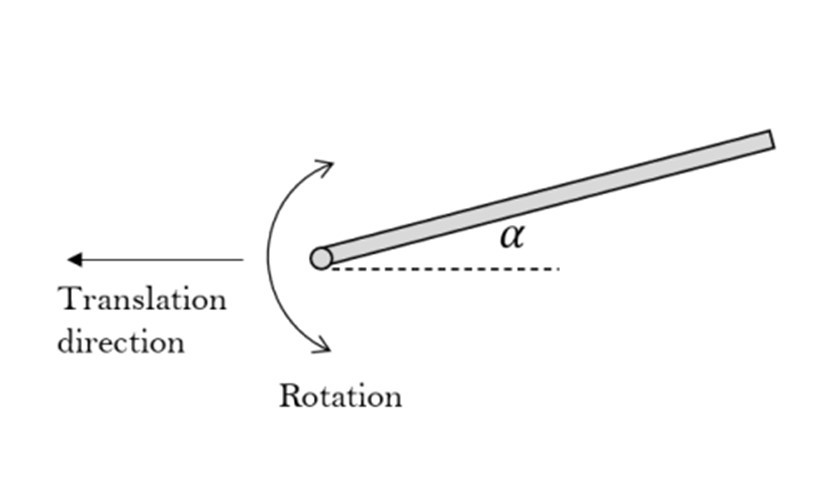
\includegraphics[width=1.0\textwidth]{graph/case1_problem_1.jpg}
        \caption{Caudal fin kinematic}
    \end{subfigure}
    \begin{subfigure}{0.4\textwidth}
        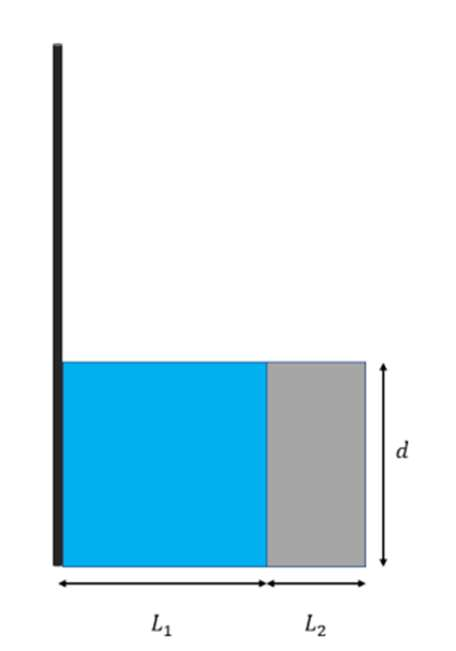
\includegraphics[width=0.5\textwidth]{graph/case1_problem_2.jpg}
        \caption{An illustration of the fin panel used in the current experiment. The length $L$ of the fin panel is 100 mm. The length of the acrylic and silicone rubber part are denoted as $L_1$ and $L_2$, respectively}
    \end{subfigure}
    \caption{\label{fig:case1_problem} Schematic of the problem}
\end{figure}

The dataset consists of 140 data points and 3 columns. The columns are the flapping frequency \texttt{flapfreq}, the acrylic percentage \texttt{percentage\_ac} indicating the stiffness, and the thrust \texttt{Thrust\_N}. For this problem, we are going to predict the thrust produced by the flapping plate given the flapping frequency and the acrylic percentage.

\paragraph{Data Inspection and Preprocessing}
First, we check null values from the data set and make sure there is no null values, which is confirmed. Next, we may calculate the Pearson correlation coefficient between each columns, as shown in \ref{fig:case1_corr_heatmap}. We can see that the magnitude of the correlation coefficient of flapping frequency on the matrix is 0.3 and the magnitude of the correlation coefficient of stiffness is 0.15. So, we know that flapping frequency is more correlated to the output rather than stiffness. However, both the magnitudes are closer to 0 which means that both variables are quite uncorrelated with the output.
\begin{figure}[H]
    \centering
    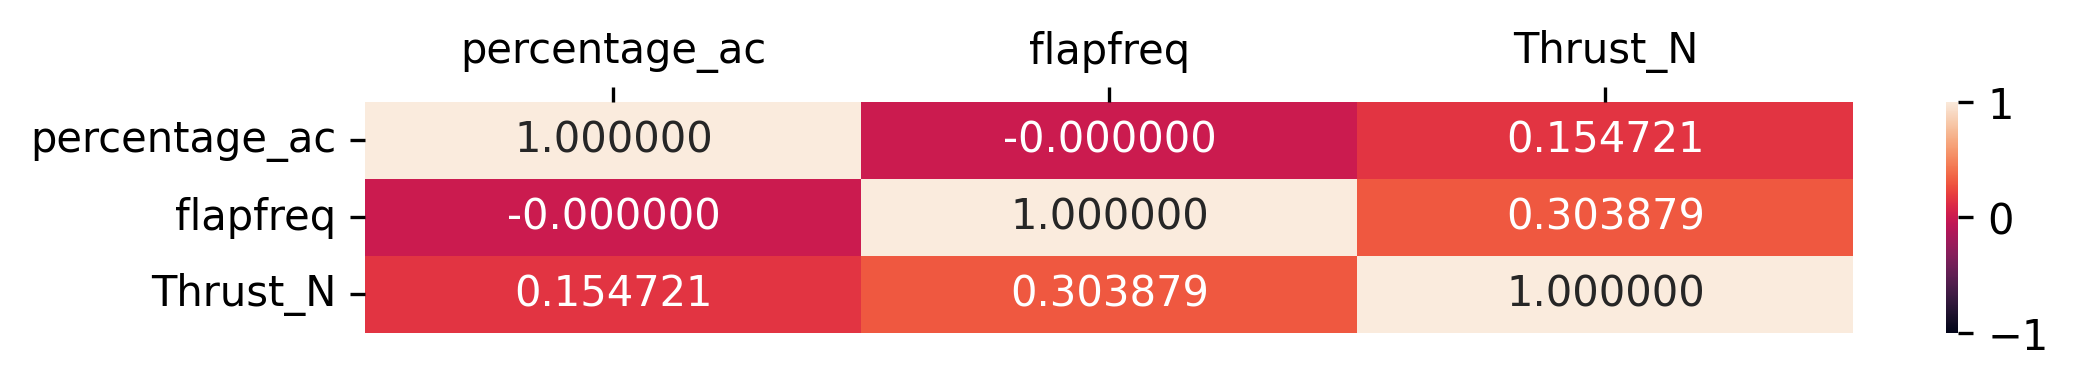
\includegraphics[width=0.75\textwidth]{graph/case1_corr_heatmap.png}
    \caption{\label{fig:case1_corr_heatmap} Pearson correlation coefficient heatmap for case 1}
\end{figure}
We may also plot the data in a 3D scatter plot, as shown in Figure \ref{fig:case1_3d_scatter}.
\begin{figure}[H]
    \centering
    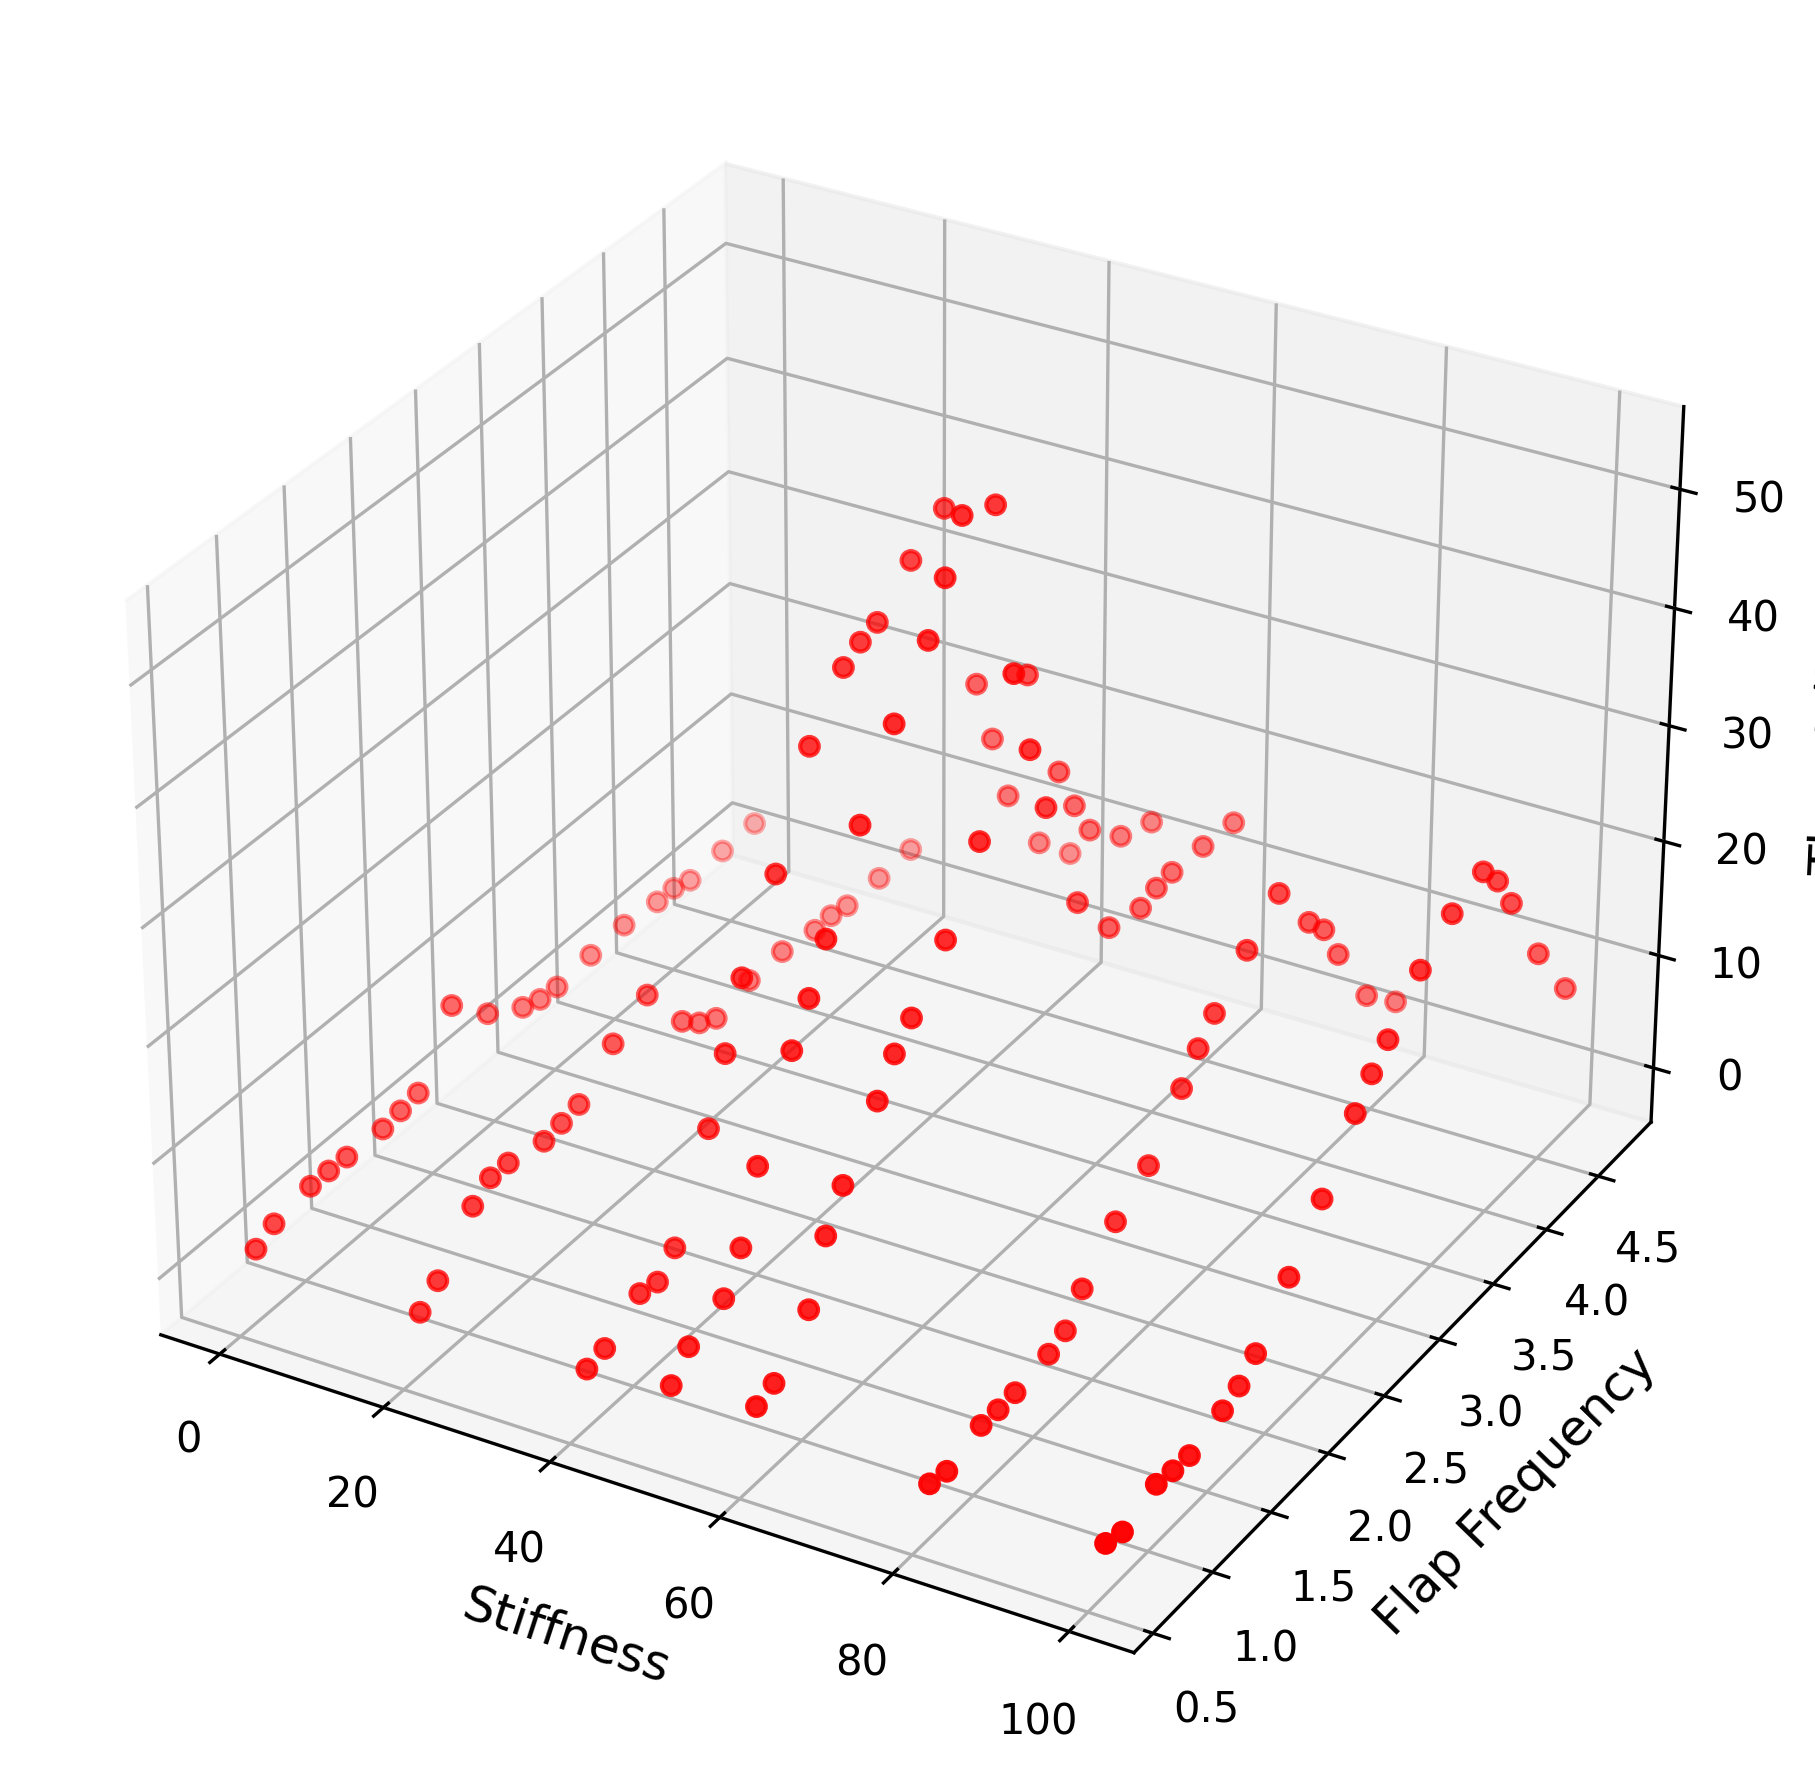
\includegraphics[width=0.5\textwidth]{graph/case1_3d_scatter.png}
    \caption{\label{fig:case1_3d_scatter} 3D scatter plot of the data in case 1}
\end{figure}
Before we train the model, we need to split the data into training and testing set. We will use 80\% of the data for training and the rest for testing. The testing set will be used to evaluate the accuracy of the model. We will use \texttt{train\_test\_split} from \texttt{sklearn.model\_selection} to split the data. 

\paragraph{Model Selection}
Here, we have to predict a continuous value, thus we will use regression models. We will use linear regression and KNN regression.

\paragraph{Model Training dan Evaluation}
\subparagraph{Linear Regression}
Using \ref{eq:betaval}, we can calculate the value of $\beta$s for linear regression. Their values including the hypothesis test is shown in Table \ref{tab:case1_beta_val}. 
We also obtained the value of $R^2$ and MSE, which are stored in Table \ref{tab:case1_r2_rse}.
\begin{table}[H]
    \centering
    \caption{\label{tab:case1_beta_val}Coefficient for Linear Regression Model in Case 1}
    \begin{tabular}{lrrrrr}
        \toprule
        Beta &      Value &  Standard Error &  $t$-statistic &   $p$-value & Hypothesis Test Result \\
        \midrule
        0 &  2.685464 &        3.355178 &     0.800394 &  0.425208 &       Do Not Reject $H_0$ \\
        1 &  0.048543 &        0.039070 &     1.242471 &  0.216705 &       Do Not Reject $H_0$ \\
        2 &  3.225045 &        0.977165 &     3.300410 &  0.001302 &              Reject $H_0$ \\
        \bottomrule
    \end{tabular}
\end{table}
\begin{table}[H]
    \centering
    \caption{\label{tab:case1_r2_rse}Coefficient of Determination and Residual Standard Error for Linear Regression Model in Case 1}
    \begin{tabular}{lr}
        \toprule
        Score Metric &      Value \\
        \midrule
        $R^2$ &      0.106227 \\
        RSE &        12.910842 \\
        \bottomrule
    \end{tabular}
\end{table}

\subparagraph{KNN Regression}
Before building the KNN model, we will scale the data based on the maximum and minimum values of the training set by using \texttt{MinMaxScaler} from \texttt{sklearn.preprocessing}, because the data distribution is not a normal but there is no outlier. The cross-validation for hyperparameter-tuning the $k$ values will be conducted with \texttt{GridSearchCV} from \texttt{sklearn.model\_selection}. Using 10-fold cross-validation, we obtained the best value of $k$ to be 2. Figure \ref{fig:case1_knn_rmse} shows the cross-validation score for each $k$ value. 
\begin{figure}[H]
    \centering
    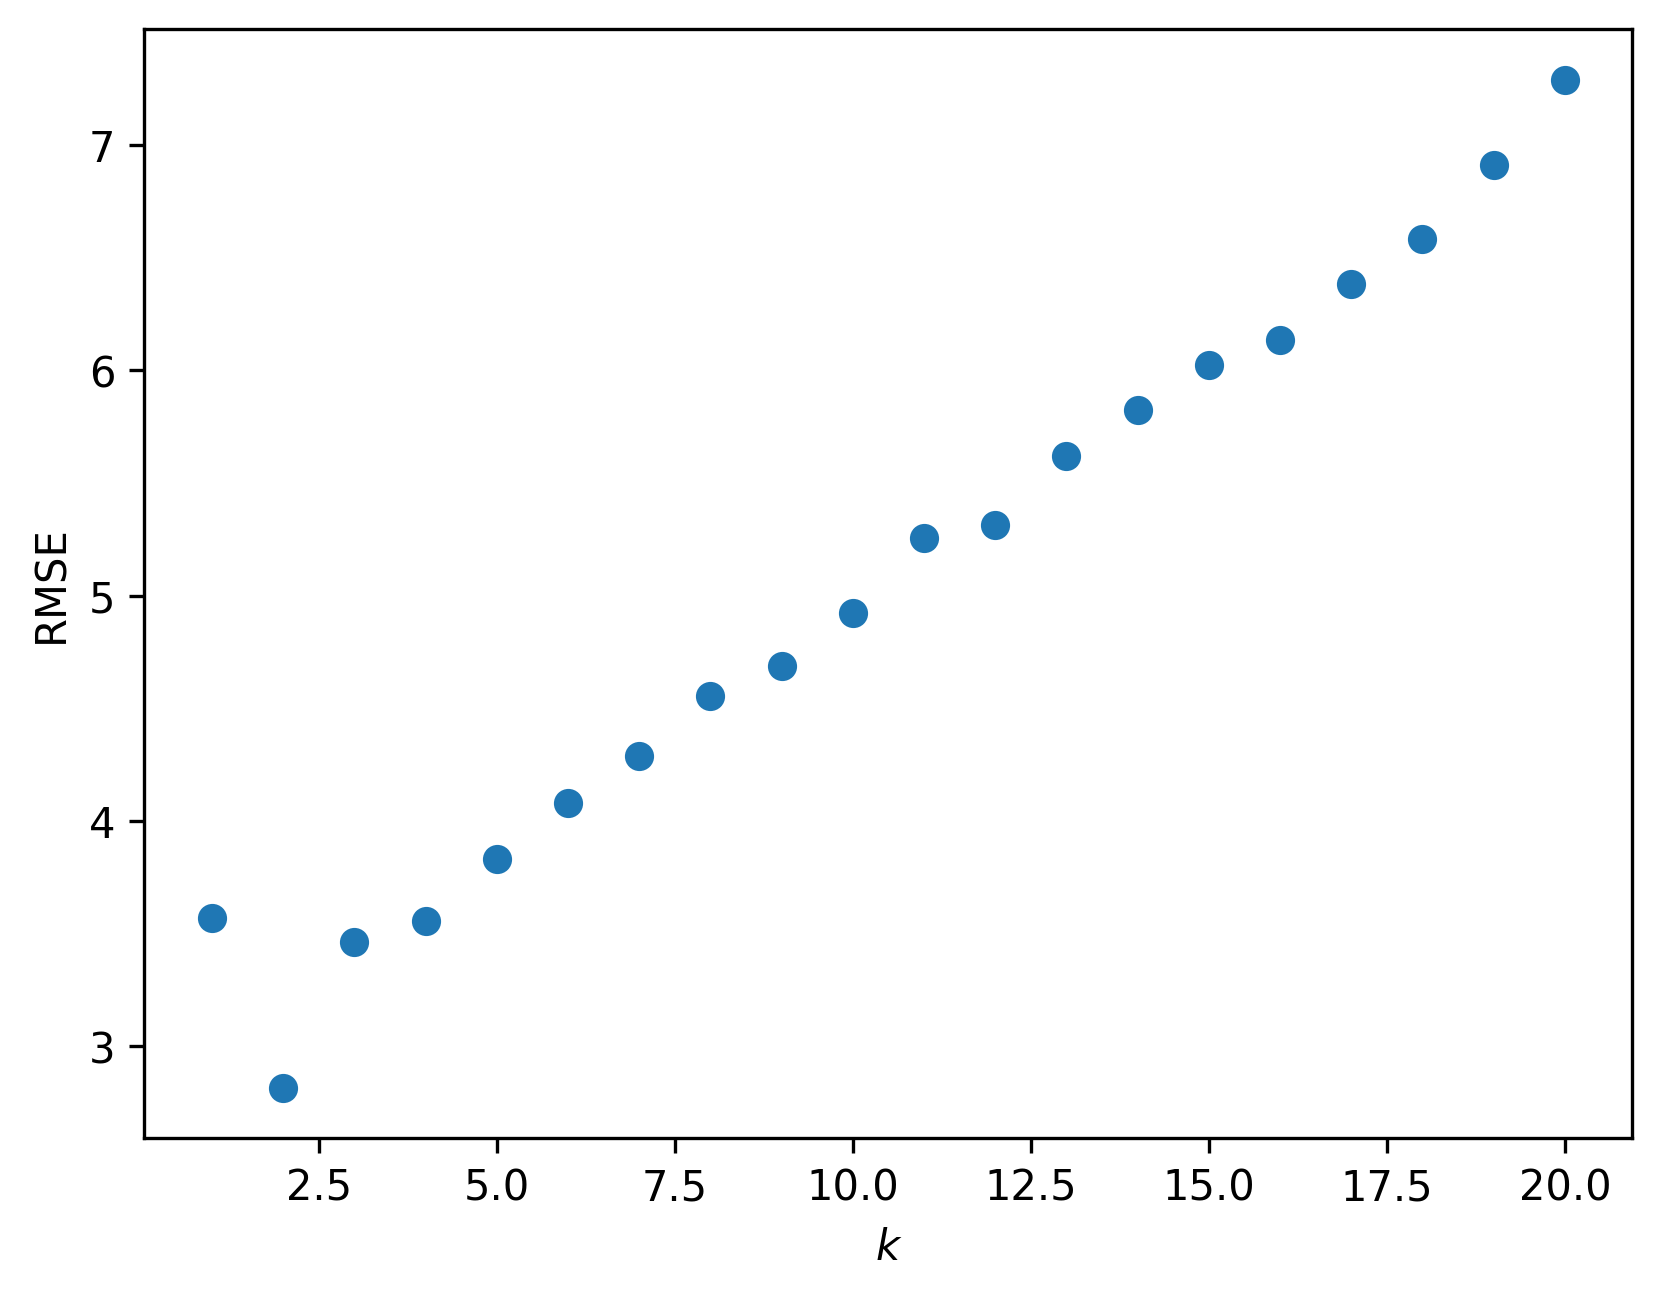
\includegraphics[width=0.5\textwidth]{graph/case1_knn_rmse.png}
    \caption{\label{fig:case1_knn_rmse} Cross-validation score for each $k$ value in case 1}
\end{figure}

\subparagraph{Model Evaluation}
We will use the testing set to evaluate the accuracy of the model, using RSME and MAE value. The result is shown in Table \ref{tab:case1_model_eval}.
\begin{table}[H]
    \centering
    \caption{\label{tab:case1_model_eval} RMSE and MAE of Linear Regression and KNN Regression in Case 3}
    \begin{tabular}{lrr}
        \toprule
        Model &      RMSE &       MAE \\
        \midrule
        Linear Regression &  11.102670 &  8.399192 \\
        KNN Regression    &  2.308239 &  1.182974 \\
        \bottomrule
    \end{tabular}
\end{table}

After comparing 2 models we created earlier, we know that RMSE and MAE values of the KNN regression model is lower than the linear regression model. From there, we can conclude that the KNN regression model better describes the approximation relationship between thrust as the output with the frequency and the stiffness as the input variables. 
Linear regression model does not fit to interpret the data set we process before can be seen from the RSE and $R^2$ score obtained, the $R^2$ score is closer to 0, it shows that data does not fit to the regression line

\paragraph{Conclusion}
From the results of calculating the coefficient of the linear regression model and the hypothesis testing in Table \ref{tab:case1_beta_val}, we can see that for $\beta_0$ and $\beta_1$, the hypothesis testing result is to do not reject $H_0$, we can interpret that the coefficients are not significant. While for $\beta_2$ the hypothesis testing result is to reject $H_0$, which means the coefficient is significant. 

The results of hypothesis testing that do not reject $H_0$ are of $\beta_0$ and $\beta_1$, where $\beta_0$ is the intercept parameter and $\beta_1$ is the coefficient of the independent variable percentage of acrylic (stiffness). Because the $H_0$ of coefficient variable stiffness is not rejected, it can be concluded that this variable is most likely unrelated to output variable (Thrust). However, there is still a relationship between the independent variable flapping frequency and output because the hypothesis results for $\beta_2$ is to reject $H_0$.

We may plot the result of both linear regression and KNN regression in a form of surface over the range of the training data, which is shown in Figure \ref{fig:case1_lr_knn_plane}.
\begin{figure}[H]
    \centering
    \begin{subfigure}{0.4\textwidth}
        \centering
        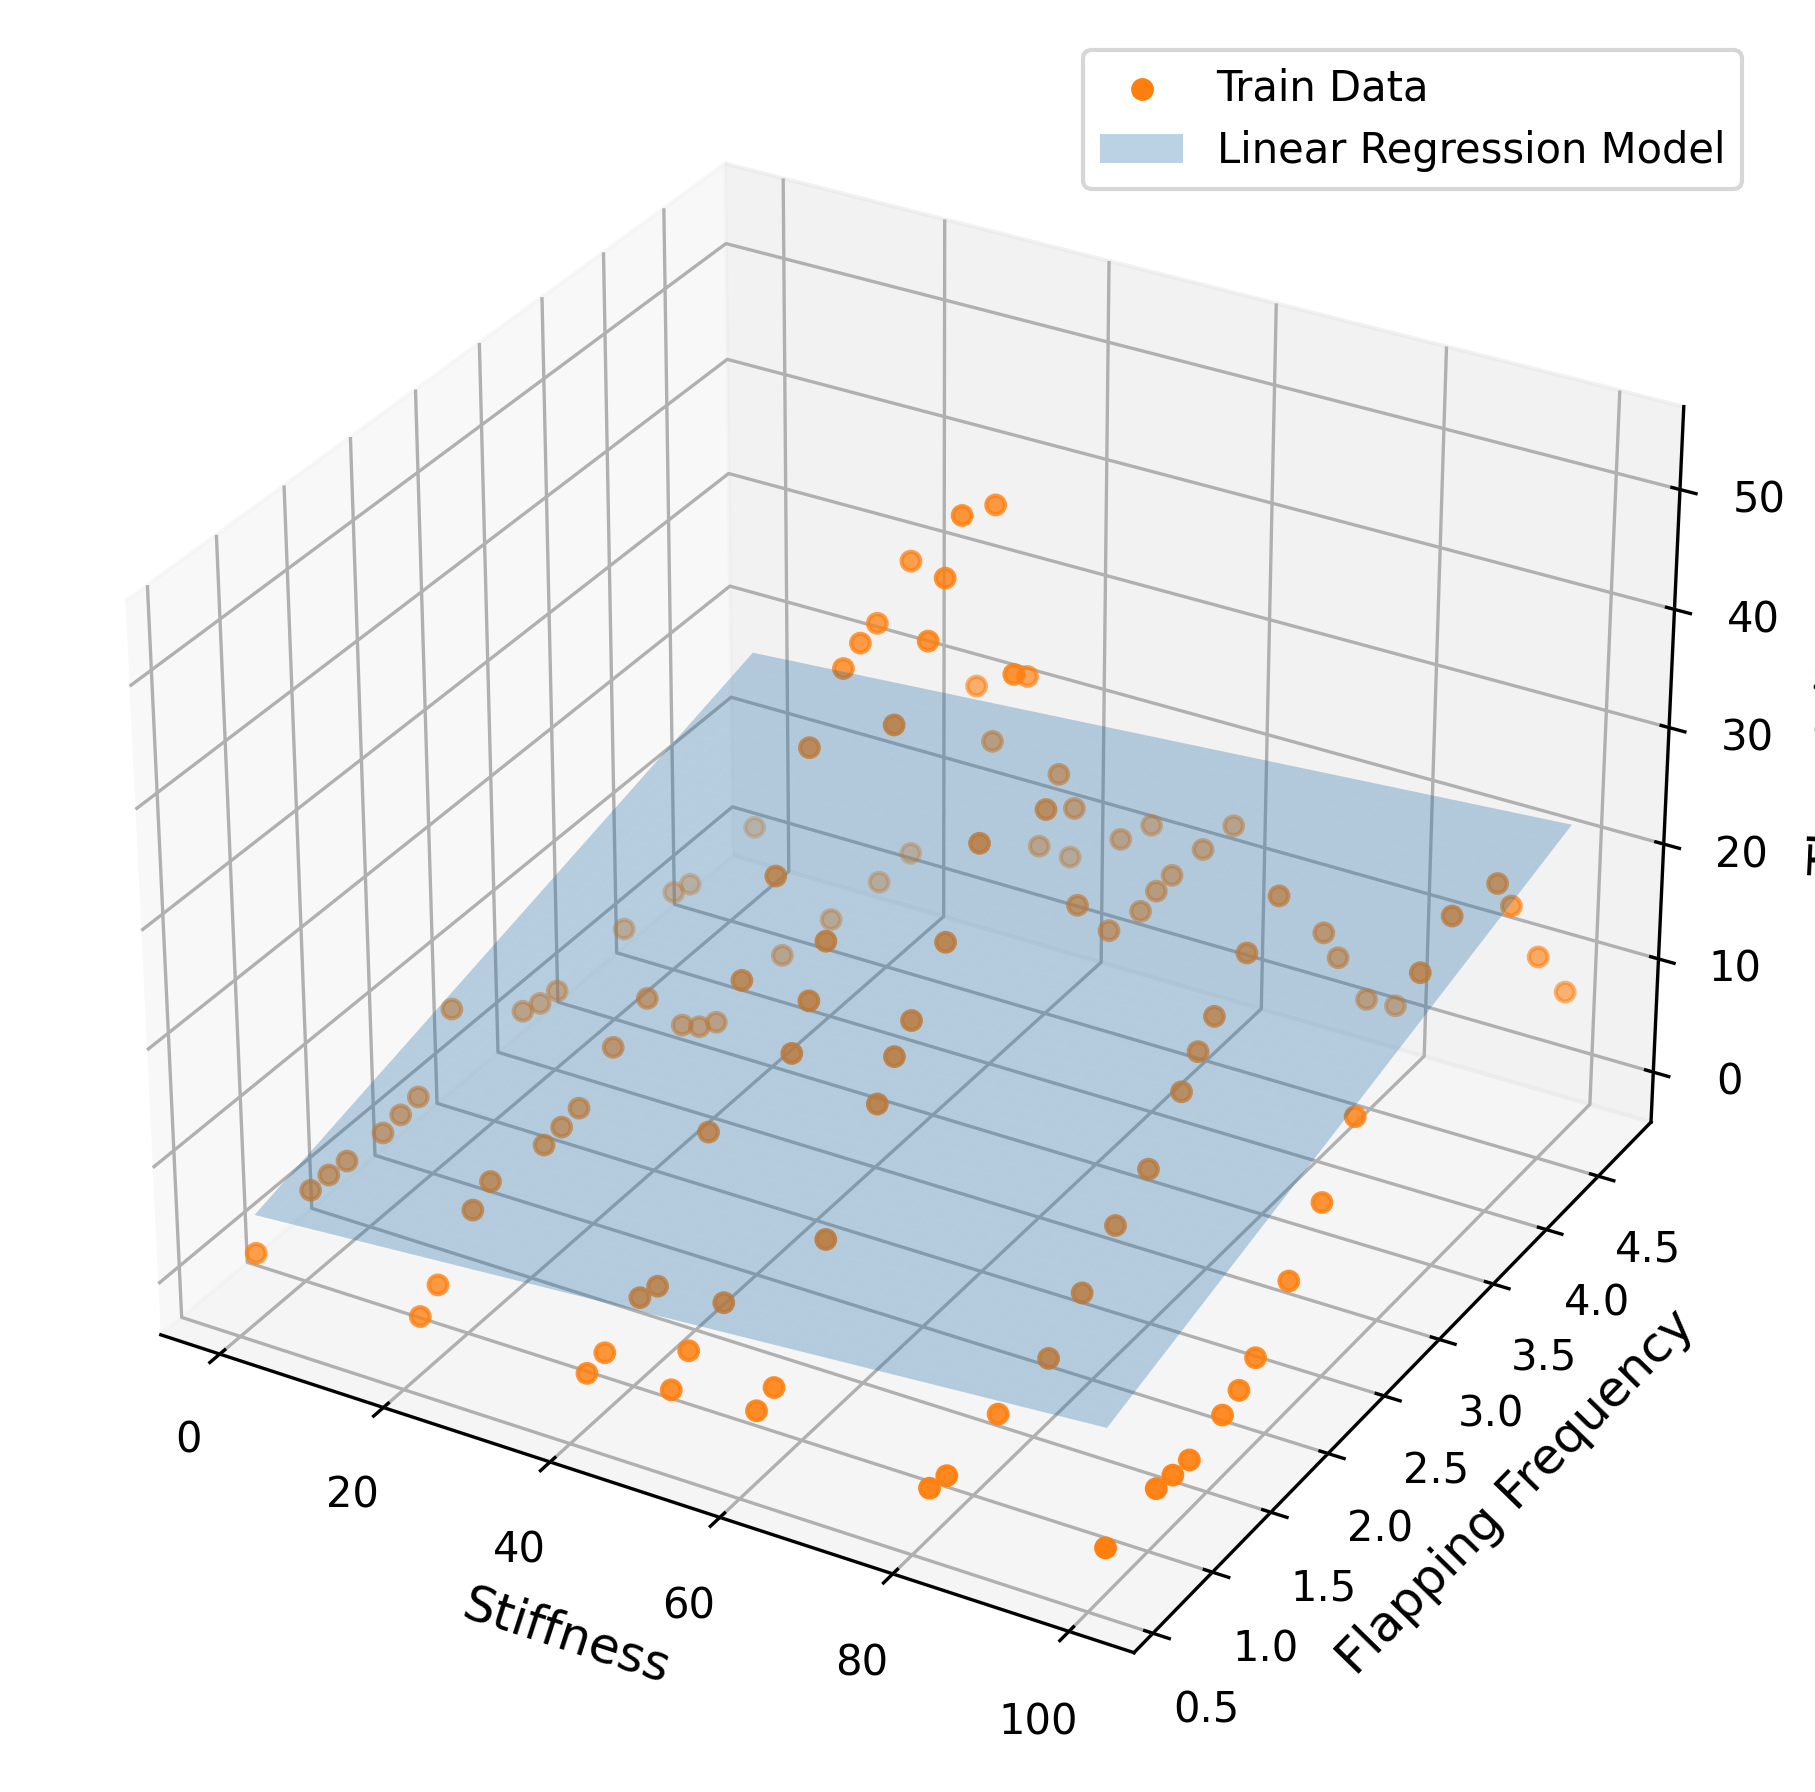
\includegraphics[width=1.0\textwidth]{graph/case1_lr_plane.png}
        \caption{Linear Regression}
    \end{subfigure}
    \hfill
    \begin{subfigure}{0.4\textwidth}
        \centering
        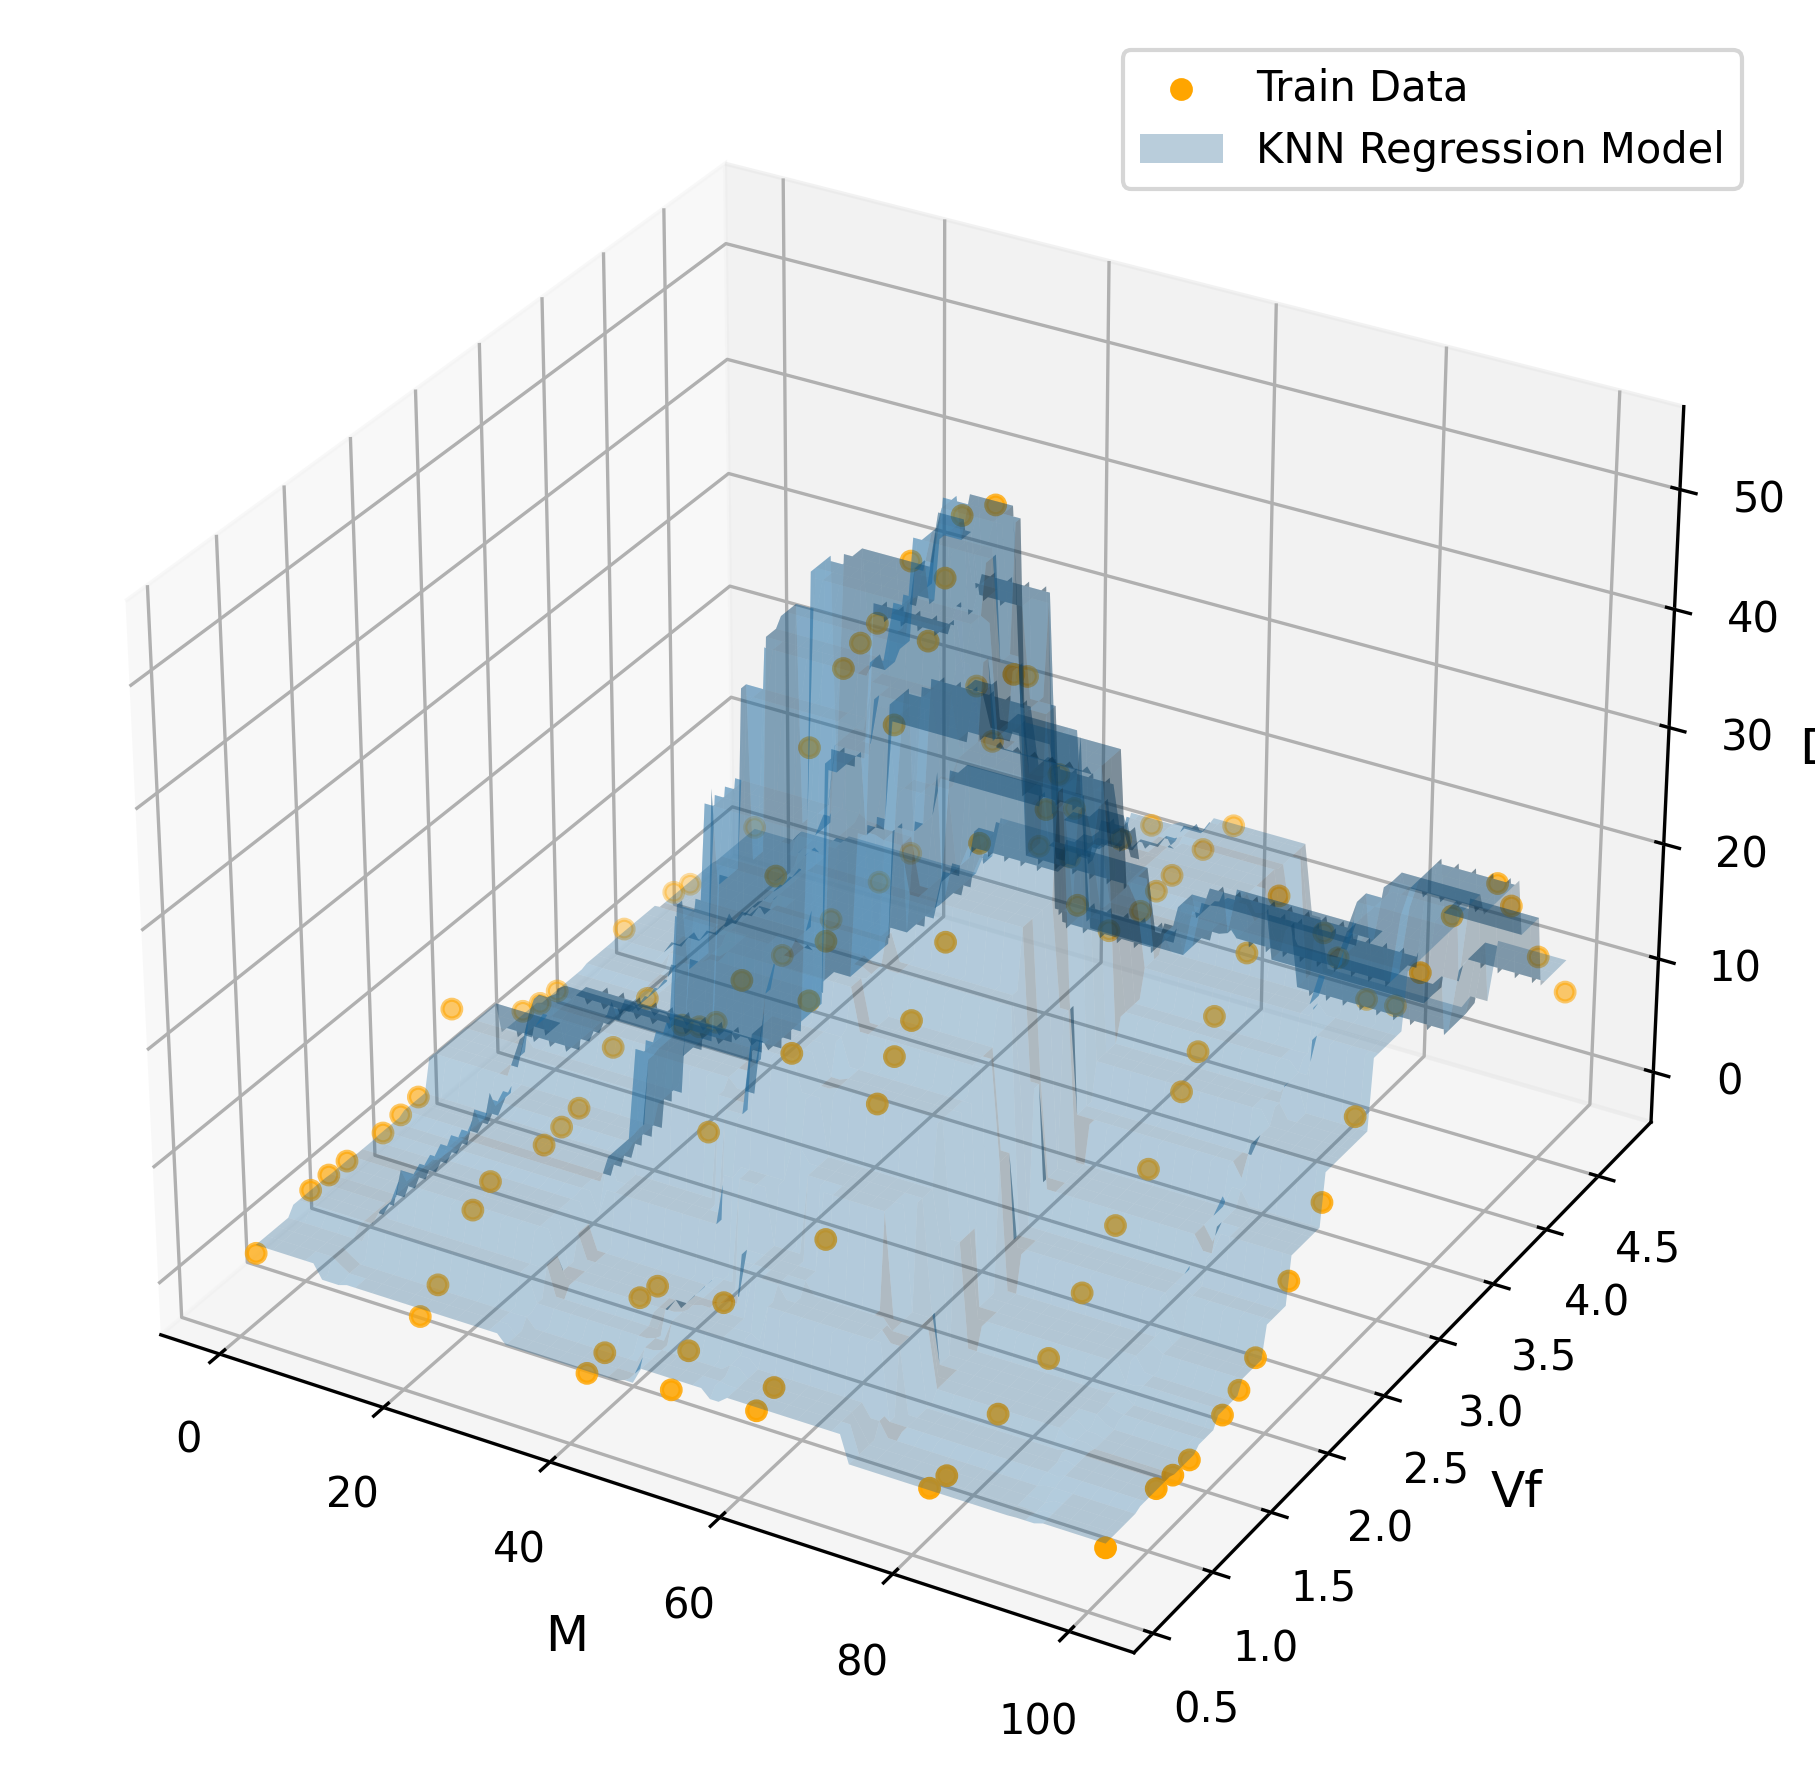
\includegraphics[width=1.0\textwidth]{graph/case1_knnr_plane.png}
        \caption{KNN Regression}
    \end{subfigure}
    \caption{\label{fig:case1_lr_knn_plane} Surface plot of the linear regression and KNN regression model in case 1}
\end{figure}


\subsection{Case 2: Aerodynamic Coefficient}
We're using data from a study investigating about the impact of transonic airfoil geometries on the drag and lift production. The airfoil is designed to operate at Mach number of 0.73 and Angle of Attack of 2 degrees. The aerodynamics coefficients are evaluated using a simplified aerodynamic solver, which neglects the viscosity of the air. 

The dataset contains 12 columns and 500 rows. The description for each column are shown in Table \ref{tab:case2_data_info}. Figure \ref{fig:case2_problem} also illustrate the parameters of the dataset. For this problem, we are going to predict the lift coefficient (\texttt{CL}) and drag coefficient (\texttt{CD}) based on the other parameters, and rank the importance of each parameter to the outputs.
\begin{table}[H]
    \centering

    \caption{\label{tab:case2_data_info}Description of Data in Case 2}
    \begin{tabular}{l|l}
        \toprule
        Column Name & Definition \\
        \midrule
        \texttt{rle} & Radius of leading edge \\
        \texttt{xup} & Upper crest absissca \\
        \texttt{yup} & Upper crest ordinate \\
        \texttt{yxxup} & Upper crest curvature \\
        \texttt{xlo} & Lower crest absissca \\
        \texttt{ylo} & Lower crest ordinate \\
        \texttt{yxxlo} & Lower crest curvature \\
        \texttt{alpha\_te} & Trailing edge direction \\
        \texttt{beta\_te} & Trailing edge wedge angle \\
        \texttt{CL} & Lift coefficient \\
        \texttt{CD} & Drag coefficient \\
        \texttt{CM} & Moment coefficient \\
        \bottomrule
    \end{tabular}
\end{table}
\begin{figure}
    \centering
    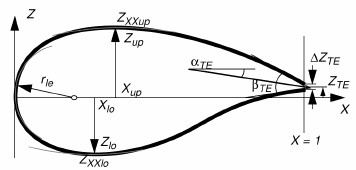
\includegraphics[width=0.5\textwidth]{graph/case2_problem.jpg}
    \caption{\label{fig:case2_problem} Illustration of the parameters in case 2}
\end{figure}


\paragraph{Data Inspection and Preprocessing}
Based on initial inspection, our dataset have a total of 500 entries, and none of them are null. Next, we may calculate the Pearson correlation parameter between each columns, as shown in Figure \ref{fig:case2_corr_heatmap}.
\begin{figure}[H]
    \centering
    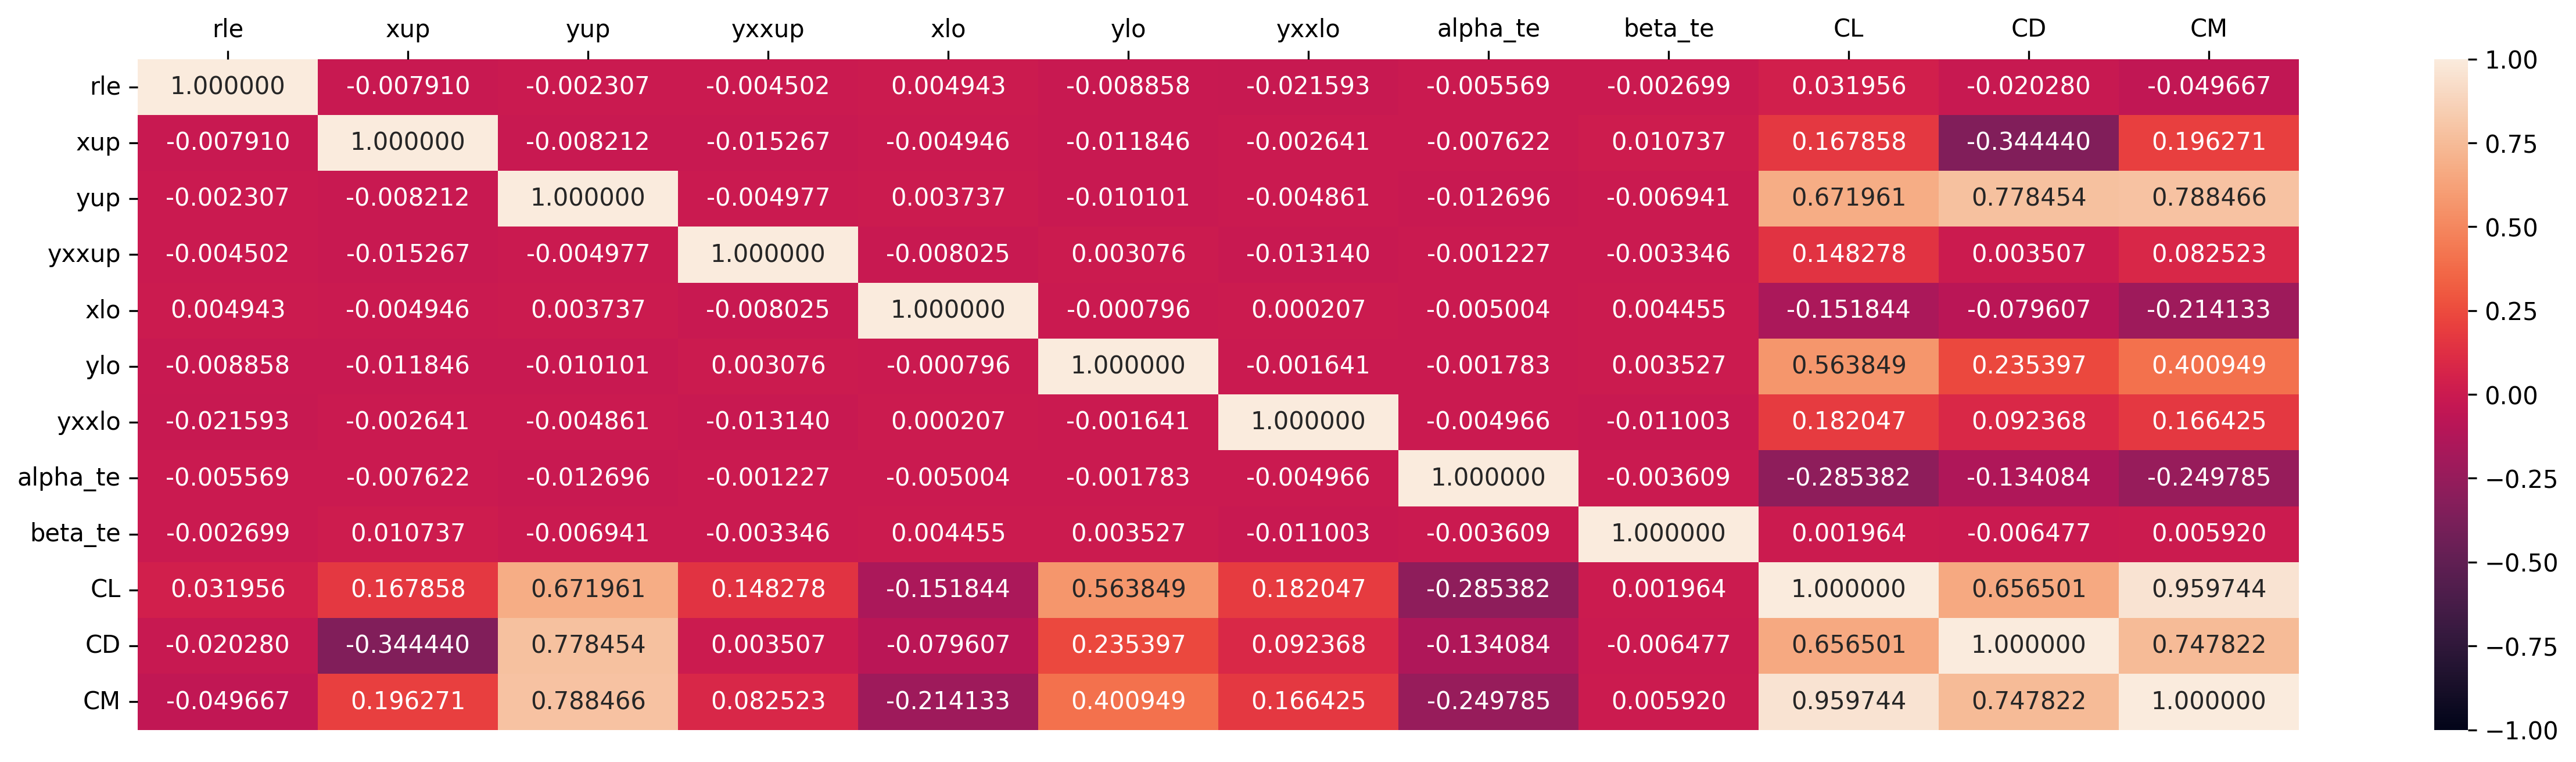
\includegraphics[width=1.0\textwidth]{graph/case2_corr_heatmap.png}
    \caption{\label{fig:case2_corr_heatmap} Pearson correlation heatmap of the parameters in case 2}
\end{figure}
Based on values shown in \ref{fig:case2_corr_heatmap}, the input variables having the strongest correlation with \texttt{CD}, \texttt{CL}, and \texttt{CM} is demonstrated by \texttt{yup}, or the upper crest ordinate.

Before we train the model, as we're going to rank the importance of each parameter, we may scale the data using \texttt{MinMaxScaler} from \texttt{sklearn.preprocessing}. We may also split the data into training and testing set, with the ratio of 80:20, using \texttt{train\_test\_split} from \texttt{sklearn.model\_selection}.

\paragraph{Model Selection}
Here, we have to predict continuous values, thus we will use regression models. We will use linear regression and KNN regression. 

\paragraph{Model Building and Evaluation}
\subparagraph{Linear Regression}
Using \eqref{eq:betaval}, we can calculate the value of $\beta$s of \texttt{CD}, \texttt{CL}, and \texttt{CM} for the linear regression model. The results including the hypothesis test is shown in Table \ref{tab:case2_beta_val}. We also evaluate the $R^2$ and RSE score of the model as shown in Table \ref{tab:case2_r2_rse}.

\begin{table}[H]
    \centering
    \caption{\label{tab:case2_beta_val} Coefficient for Linear Regression Model in Case 2}
    \begin{subtable}{1.0\textwidth}
        \centering
        \caption{Coefficient for Linear Regression of \texttt{CD}}
        \begin{tabular}[width=1.0\textwidth]{lrrrrr}
            \toprule
            Beta &      Values &  Standard Error &  $t$-statistic &        $p$-value & Hypothesis Test Result \\
            \midrule
            0 &  0.003348 &        0.000917 &     3.650961 &   2.967747e-04 &              Reject H0 \\
            1 & -0.000122 &        0.000574 &    -0.212497 &   8.318299e-01 &       Do Not Reject H0 \\
            2 & -0.008557 &        0.000575 &   -14.881558 &   5.263659e-40 &              Reject H0 \\
            3 &  0.019872 &        0.000572 &    34.719043 &  1.666999e-121 &              Reject H0 \\
            4 & -0.000251 &        0.000570 &    -0.440322 &   6.599476e-01 &       Do Not Reject H0 \\
            5 & -0.001914 &        0.000577 &    -3.315638 &   9.998077e-04 &              Reject H0 \\
            6 &  0.006563 &        0.000580 &    11.320195 &   6.876674e-26 &              Reject H0 \\
            7 &  0.002742 &        0.000570 &     4.809075 &   2.167568e-06 &              Reject H0 \\
            8 & -0.003241 &        0.000570 &    -5.684308 &   2.572116e-08 &              Reject H0 \\
            9 &  0.000050 &        0.000568 &     0.088217 &   9.297497e-01 &       Do Not Reject H0 \\
            \bottomrule
        \end{tabular}
    \end{subtable}
    \vskip \baselineskip
    \begin{subtable}{1.0\textwidth}
        \centering
        \caption{Coefficient for Linear Regression of \texttt{CL}}
        \begin{tabular}[width=1.0\textwidth]{lrrrrr}
            \toprule
            Beta &      Values &  Standard Error &  $t$-statistic &        $p$-value & Hypothesis Test Result \\
            \midrule
            0 &  0.521795 &        0.005601 &    93.166063 &  4.622280e-269 &              Reject H0 \\
            1 &  0.015680 &        0.003507 &     4.471338 &   1.019951e-05 &              Reject H0 \\
            2 &  0.071101 &        0.003511 &    20.248937 &   7.215814e-63 &              Reject H0 \\
            3 &  0.263018 &        0.003495 &    75.250845 &  1.013006e-234 &              Reject H0 \\
            4 &  0.058669 &        0.003483 &    16.842160 &   2.998194e-48 &              Reject H0 \\
            5 & -0.058992 &        0.003525 &   -16.734515 &   8.600908e-48 &              Reject H0 \\
            6 &  0.220595 &        0.003540 &    62.308767 &  3.810448e-205 &              Reject H0 \\
            7 &  0.075028 &        0.003482 &    21.547331 &   1.905243e-68 &              Reject H0 \\
            8 & -0.104502 &        0.003482 &   -30.015382 &  1.611219e-103 &              Reject H0 \\
            9 &  0.000270 &        0.003466 &     0.077996 &   9.378711e-01 &       Do Not Reject H0 \\
            \bottomrule
        \end{tabular}
    \end{subtable}
    \vskip \baselineskip
    \begin{subtable}{1.0\textwidth}
        \centering
        \caption{Coefficient for Linear Regression of \texttt{CM}}
        \begin{tabular}[width=1.0\textwidth]{lrrrrr}
            \toprule
            {} &      Beta &  Standard Error &  $t$-statistic &        $p$-value & Hypothesis Test Result \\
            \midrule
            0 &  0.045960 &        0.001605 &    28.634104 &   5.149599e-98 &              Reject H0 \\
            1 & -0.004924 &        0.001005 &    -4.899170 &   1.411907e-06 &              Reject H0 \\
            2 &  0.026385 &        0.001006 &    26.219789 &   3.620143e-88 &              Reject H0 \\
            3 &  0.100599 &        0.001002 &   100.431480 &  2.655315e-281 &              Reject H0 \\
            4 &  0.010215 &        0.000998 &    10.232636 &   6.212311e-22 &              Reject H0 \\
            5 & -0.026673 &        0.001010 &   -26.402278 &   6.382478e-89 &              Reject H0 \\
            6 &  0.052365 &        0.001015 &    51.611323 &  1.240393e-176 &              Reject H0 \\
            7 &  0.022564 &        0.000998 &    22.611134 &   5.382271e-73 &              Reject H0 \\
            8 & -0.029863 &        0.000998 &   -29.929553 &  3.518305e-103 &              Reject H0 \\
            9 &  0.000521 &        0.000993 &     0.524790 &   6.000263e-01 &       Do Not Reject H0 \\
            \bottomrule
        \end{tabular}
    \end{subtable}
\end{table}
\begin{table}[H]
    \centering
    \caption{\label{tab:case2_r2_rse}Coefficient of Determination and Residual Standard Error for Linear Regression Model in Case 2}
    \begin{tabular}[width=1.0/textwidth]{lrrr}
        \toprule
        Score Metric &      \texttt{CD} & \texttt{CL} & \texttt{CM} \\
        \midrule
        $R^2$ &      0.808617 & 0.967612 & 0.975402 \\
        RSE &        0.003305 & 0.020183 & 0.005784 \\
        \bottomrule
    \end{tabular}
\end{table}

We may now evalute the linear regression model using $R^2$ and $RSE$ score for each aerodynamic coefficients from \ref{tab:case2_r2_rse}.
\begin{enumerate}
    \item \texttt{CD}
    
    From the table, we can see that the obtained value of $R^2$ is 0.808617. This translates to roughly 81\% variance in the model is explained by the model. In engineering, preceding $R^2$ value is considered good and shows strong correlation between input and output. Therefore, the model is viable for making future predictions.
    \item \texttt{CL}
    
    From the table, we can see that the obtained value of $R^2$ is 0.967612. This translates to roughly 97\% variance in the model is explained by the model. This $R^2$ value is considered good and shows strong correlation between input and output and therefore, the model is viable for making future predictions.
    \item \texttt{CM}
    
    From the table, we can see that the obtained value of $R^2$ is 0.975402. This translates to roughly 98\% variance in the model is explained by the model. Same as previous coefficients, the $R^2$ value is considered good and shows strong correlation between input and output, making the model is viable for making future predictions.
\end{enumerate}

\subparagraph{KNN Regression}
As the data has been scaled, we may continue directly to the model building. We will also conduct a grid search to find the $k$ value for the KNN regression model, using \texttt{GridSearchCV} from \texttt{sklearn.model\_selection}. With 5-fold cross validation, we obta

\subparagraph{Model Evaluation}

\paragraph{Conclusion}

\subsection{Case 3: Wing Flutter}
We're using the data from \cite{palar2023kernel} about flutter detection on NACA 64A10 airfoil. The dataset consist of 300 data points and 3 columns. The columns are the Mach number \texttt{M}, the flutter speed \texttt{Vf}, and the damping coefficient \texttt{DC}. For this problem, we are going predict the occurence of flutter, that is, whether the damping coefficient is positive or negative, given the Mach number and the flutter speed. A negative damping coefficient indicates that the airfoil is unstable and will flutter, and vice versa.

\paragraph{Data Inspection and Preprocessing}
Based on initial inspection, our dataset have a total of 300 entries, and none of them are null. Moreover, all of the columns are numerical, with general information stored in Table \ref{tab:case3_data_info}. 
\begin{table}[H]
    \centering
    \caption{ \label{tab:case3_data_info}General Statistics of Data in Case 3}
    \begin{tabular}{lrrr} 
        \toprule
        {} &           \texttt{M} &          \texttt{Vf} &          \texttt{DC} \\
        \midrule
        count &  300.000000 &  300.000000 &  300.000000 \\
        mean  &    0.768178 &    1.145337 &   -0.005795 \\
        std   &    0.092958 &    0.482497 &    0.039937 \\
        min   &    0.600000 &    0.400000 &   -0.104256 \\
        25\%   &    0.687750 &    0.723500 &   -0.032059 \\
        50\%   &    0.772000 &    1.100000 &   -0.000651 \\
        75\%   &    0.858500 &    1.554500 &    0.023531 \\
        max   &    0.905000 &    2.000000 &    0.095338 \\
        \bottomrule
    \end{tabular}
\end{table}
and the Pearson correlation coefficient between each columns are shown in Figure \ref{fig:case3_corr_heatmap}.
\begin{figure}[H]
    \centering
    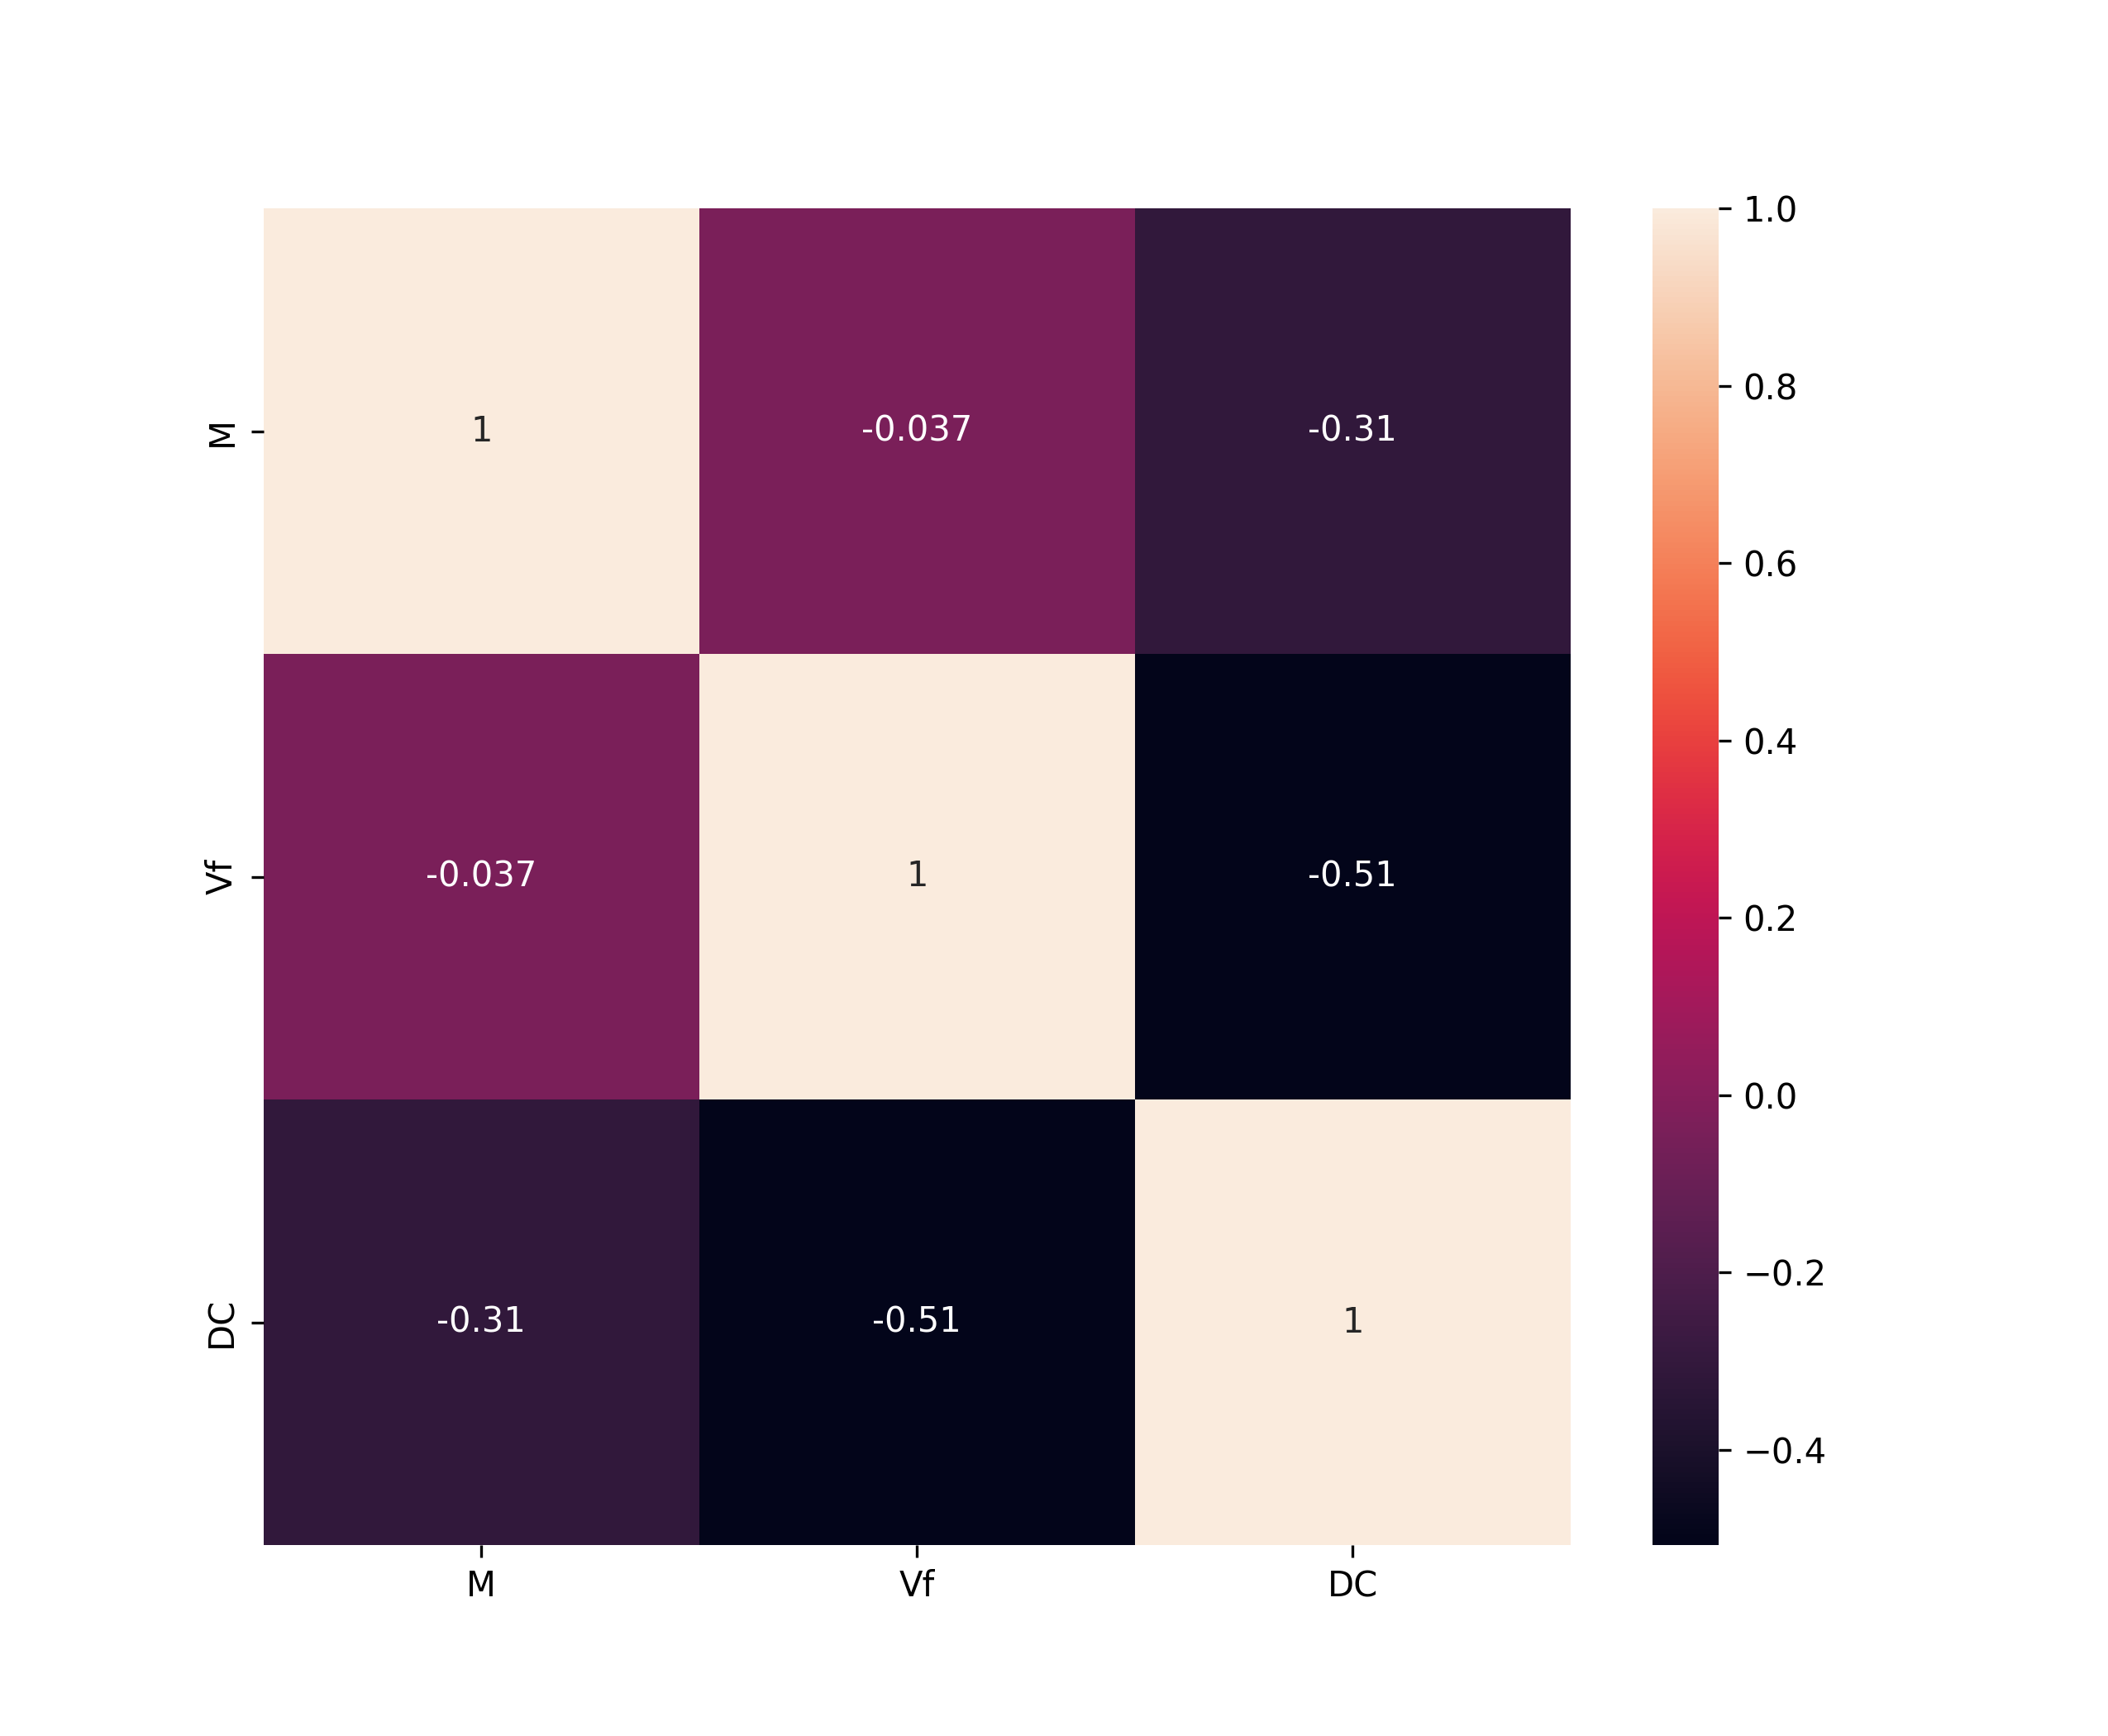
\includegraphics[width=0.75\textwidth]{graph/case3_corr_heatmap.png}
    \caption{Pearson correlation coefficient for case 3}
    \label{fig:case3_corr_heatmap}
\end{figure}
We're given a set of numerical data, but we need to predict a categorical values. Therefore, we may add a new column, named \texttt{F}, which indicates whether the airfoil will flutter or not. We can see the distribution of the data in Figure \ref{fig:case3_data_dist}.
\begin{figure}
    \centering
    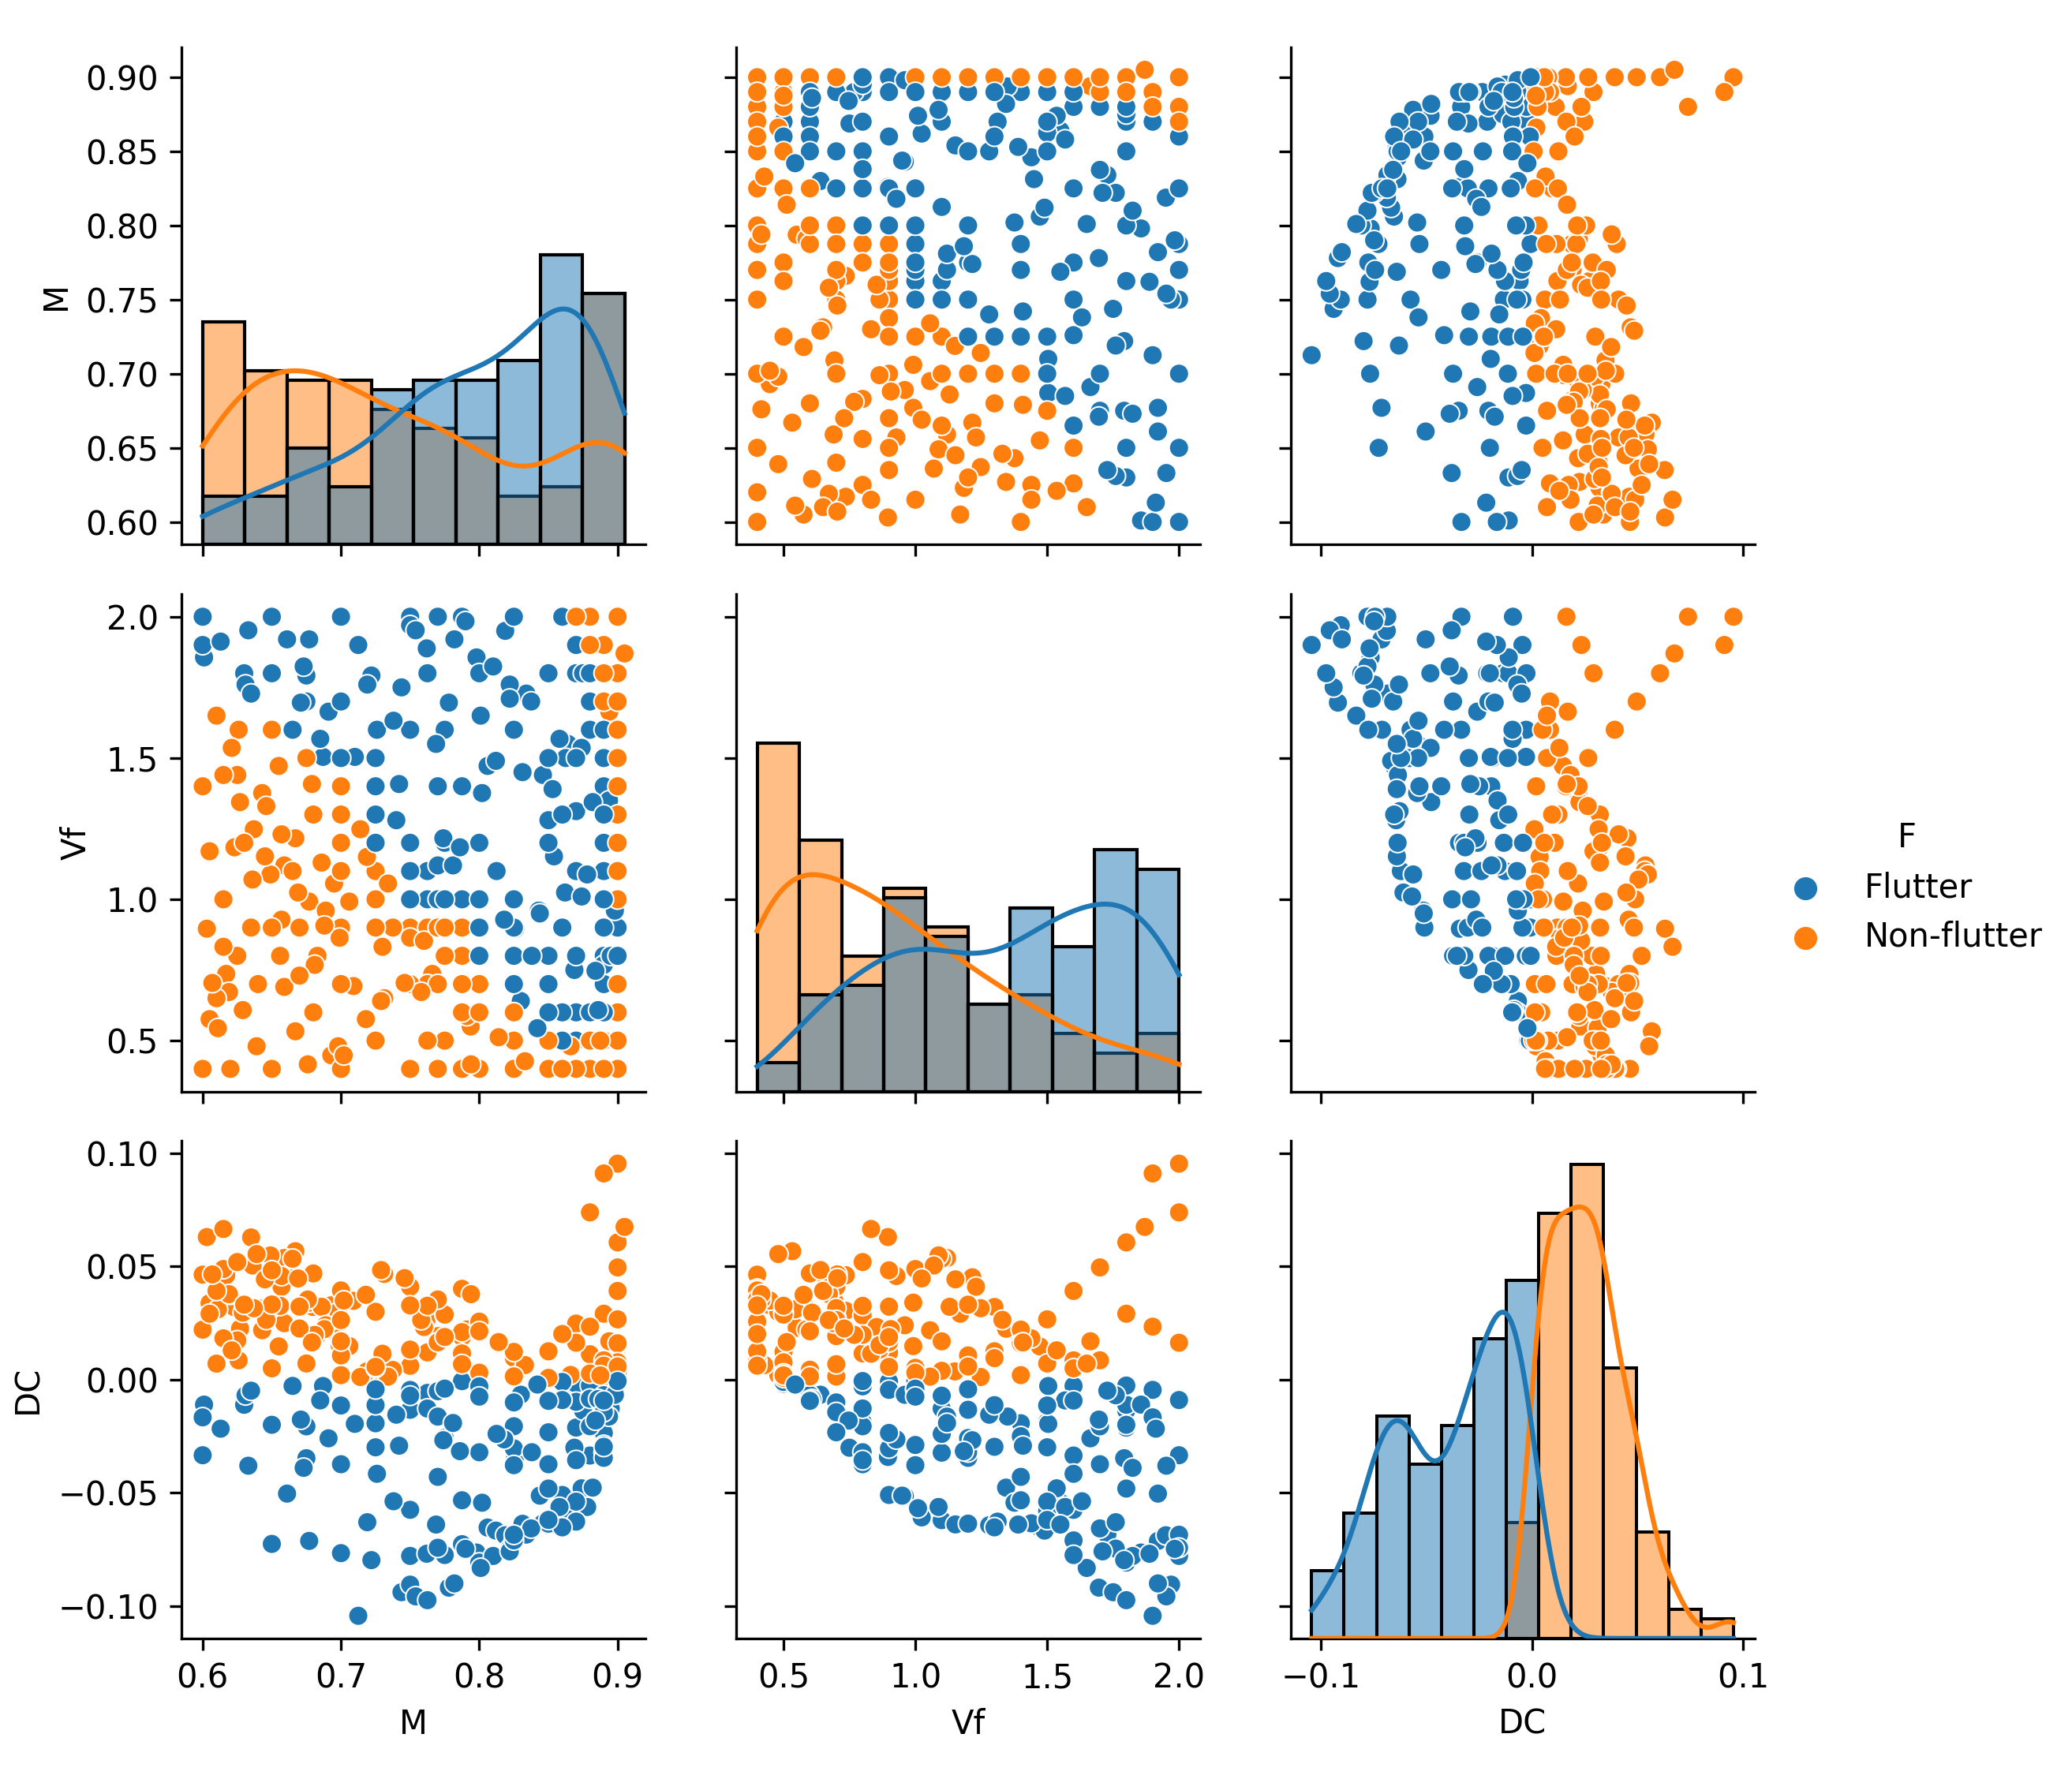
\includegraphics[width=0.8\textwidth]{graph/case3_data_dist_hue.png}
    \caption{Distribution of the data in case 3}
    \label{fig:case3_data_dist}
\end{figure}
Moreover, as we have only two inputs and an output, we may plot the data in a 3D scatter plot, as shown in Figure \ref{fig:case3_3d_scatter}.
\begin{figure}
    \centering
    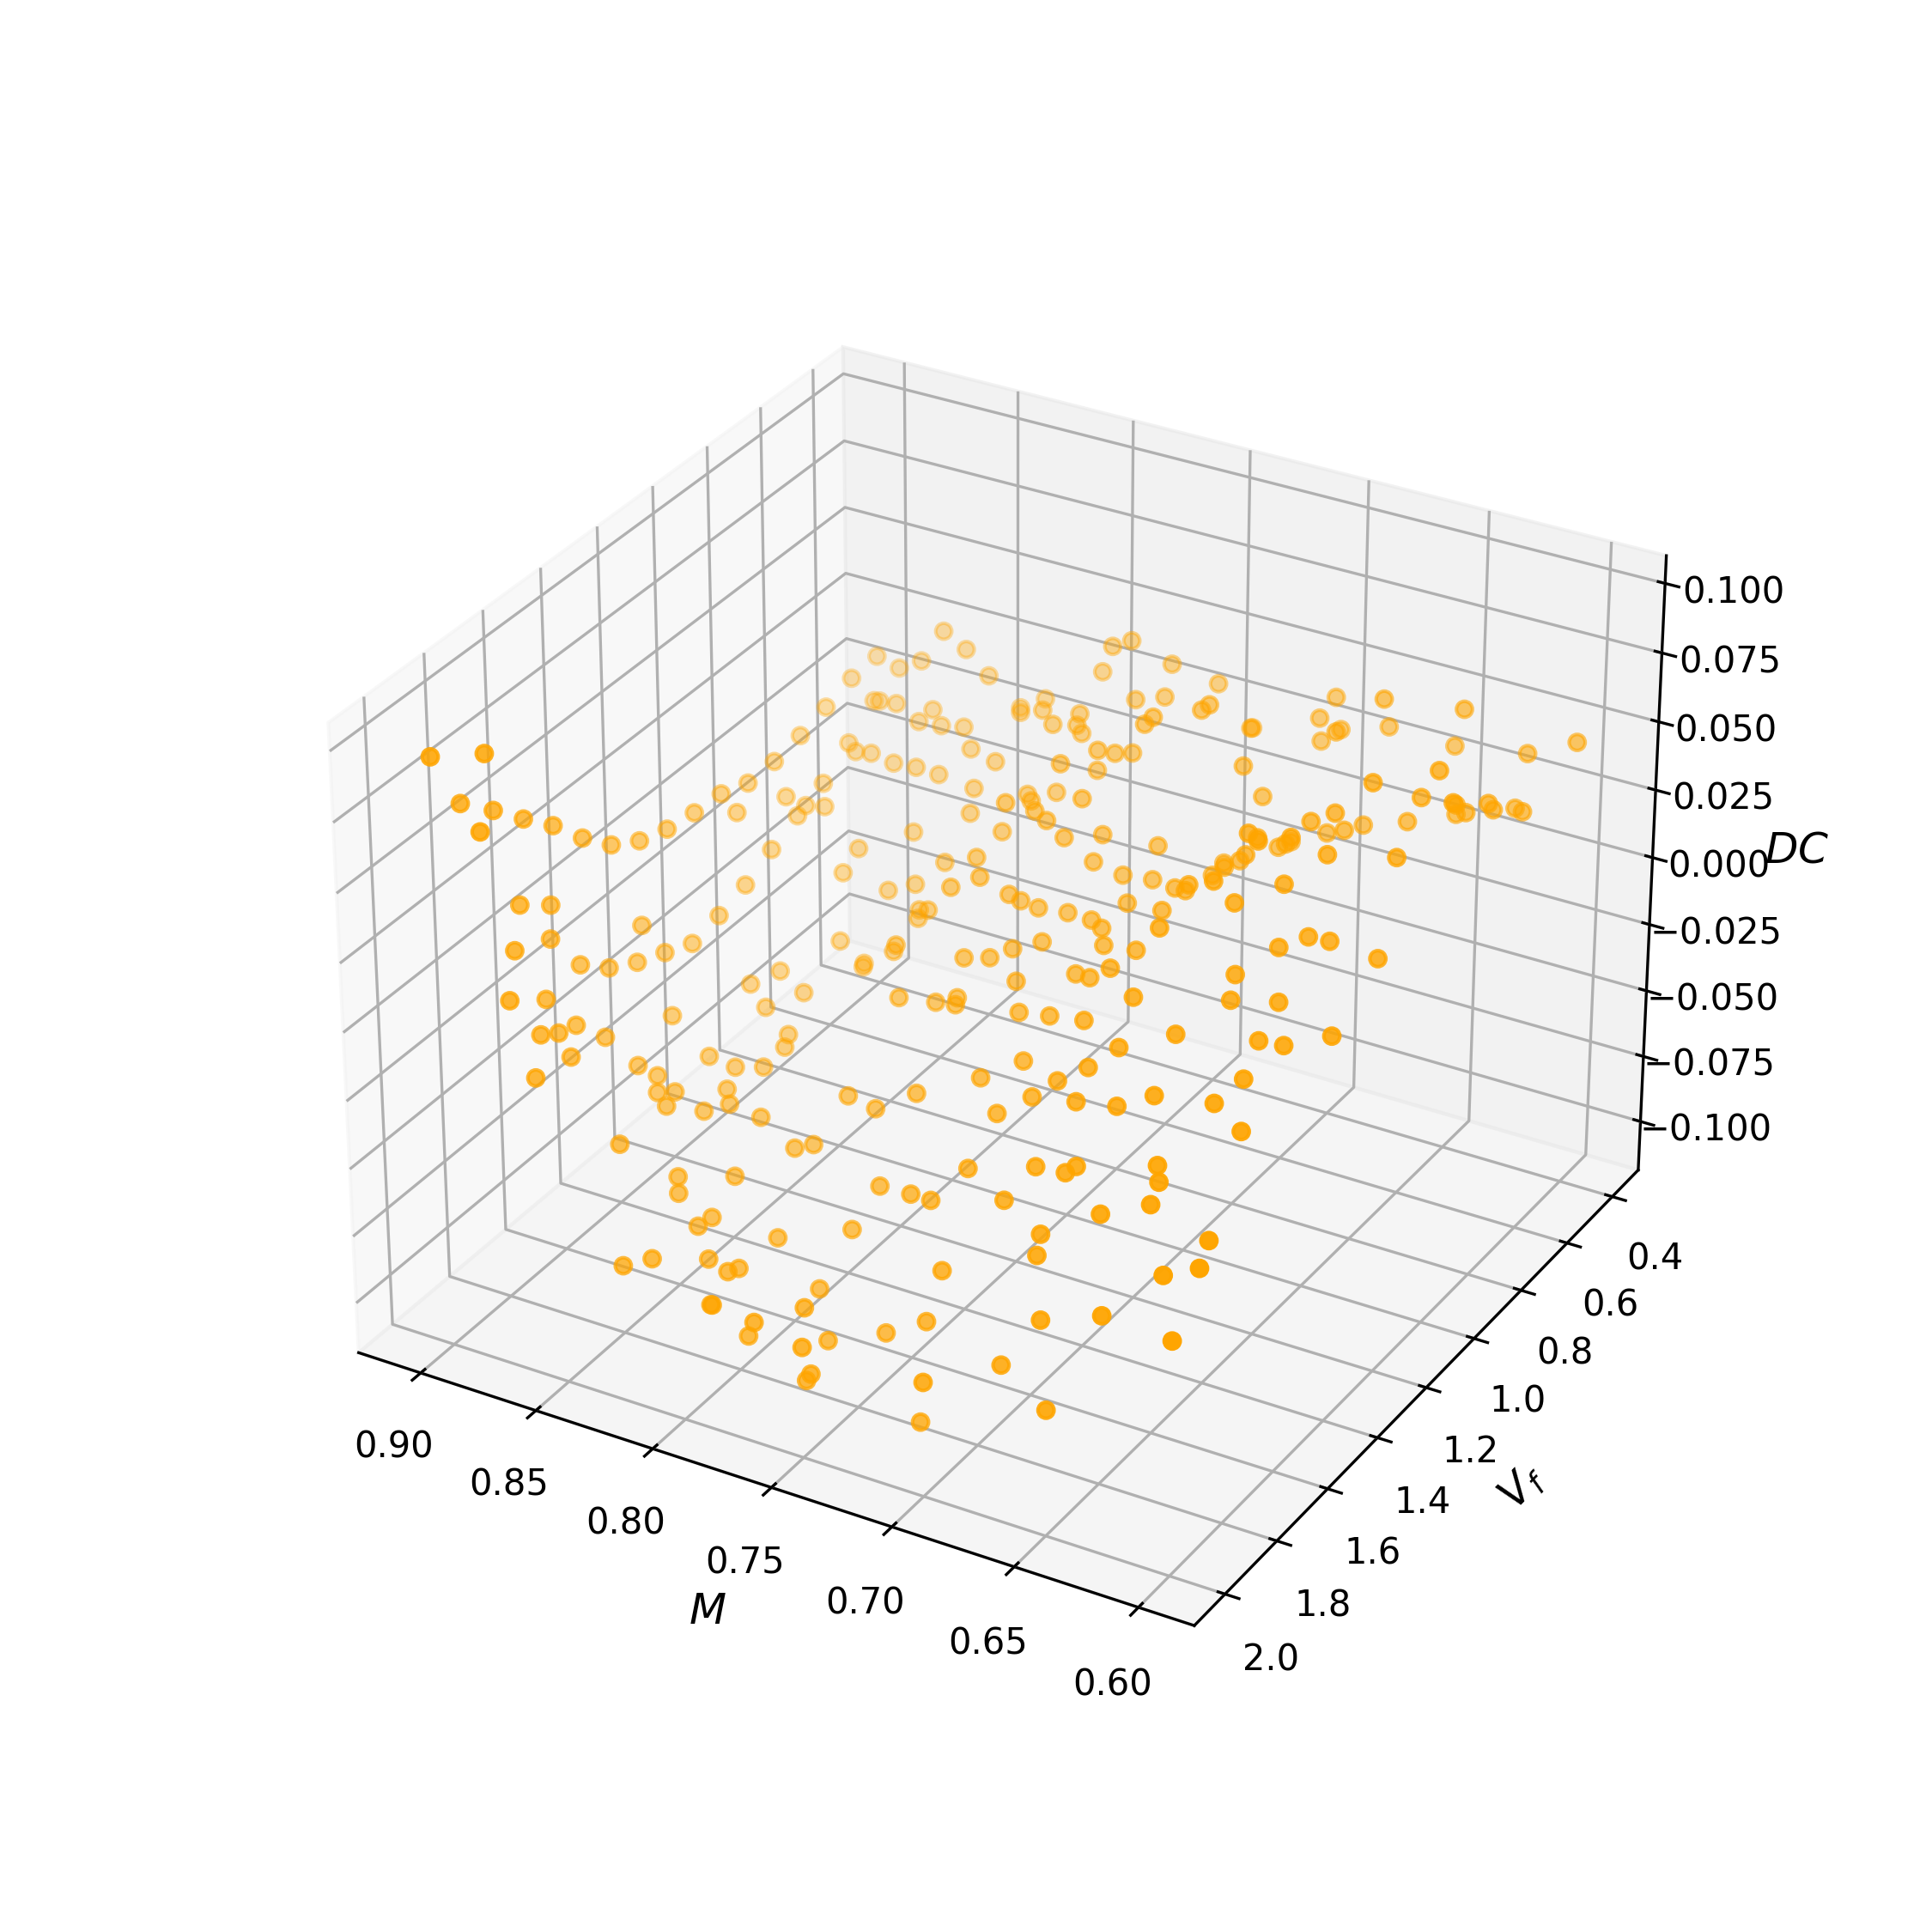
\includegraphics[width=0.5\textwidth]{graph/case3_3d_scatter.png}
    \caption{3D scatter plot of the sample data in case 3}
    \label{fig:case3_3d_scatter}
\end{figure}
From Figure \ref{fig:case3_3d_scatter}, we can see that high Mach number and high flutter speed is dominated by negative damping coefficient, which means that the airfoil will flutter. This is also supported by the correlation coefficient in Table \ref{fig:case3_corr_heatmap}, which shows that the damping coefficient is negatively correlated with both Mach number and flutter speed. From Table \ref{fig:case3_corr_heatmap}, we can see that the Mach number and flutter speed correlation coefficient is very small, which means that they are more likely to be independent with each other. We can also see the correlation between damping coefficient and other variables, which shows that the damping coefficient not quite correlated with the others, but it is more correlated with flutter speed than Mach number.

Before we train the model, we need to split the data into training and testing set. We will use 80\% of the data for training and the rest for testing. The testing set will be used to evaluate the accuracy of the model. We will use \texttt{train\_test\_split} from \texttt{sklearn.model\_selection} to split the data. 

\paragraph{Model Selection}
Here, we have to predict a categorical value, so it's quite intuitive if we use a classification model. However, the classification of our target/response, \texttt{F}, is based on value of another column, \texttt{DC}, which can be predicted using a regression model. Therefore, we will use two approach in solving this problem:
\begin{enumerate}
    \item Predict \texttt{DC} using a regression model, then obtain \texttt{F} by classifying the result manually.
    \item Predict \texttt{F} using a classification model.
\end{enumerate}

\paragraph{Model Training and Evaluation}
For both KNN algorithm, we will use \texttt{KNearestRegressor} and \texttt{KNearestClassifier} from \texttt{sklearn.neighbors}. Also, before building the KNN model, we will scale the data based on the maximum and minimum values of the training set by using \texttt{MinMaxScaler} from \texttt{sklearn.preprocessing}, because the data distribution is not a normal but there is no outlier. The cross-validation for hyperparameter-tuning the $k$ values will be conducted with \texttt{GridSearchCV} from \texttt{sklearn.model\_selection}. 

\subparagraph{Regression Model} We will use linear regression and KNN regression to predict the damping coefficient. Using \eqref{eq:betaval}, the resulting coefficient for the linear regression model and the hypothesis testing is shown in Table \ref{tab:case3_beta_val}. We can see that all $H_0$ is rejected and thus, all of the coefficients are significant. 
\begin{table}[H]
    \centering
    \caption{\label{tab:case3_beta_val}Coefficient for Linear Regression Model in Case 3}
    \begin{tabular}{lrrrrr}
        \toprule
        Beta &      Value &  Standard Error &  $t$-statistic &       $p$-value & Hypothesis Test Result \\
        \midrule
        0 &  0.158557 &        0.017985 &     8.816034 &  2.555677e-16 &              Reject $H_0$ \\
        1 & -0.145096 &        0.022156 &    -6.548710 &  3.543494e-10 &              Reject $H_0$ \\
        2 & -0.046859 &        0.004335 &   -10.808856 &  2.045755e-22 &              Reject $H_0$ \\
        \bottomrule
    \end{tabular}
\end{table}
With this model, we obtained $R^2$ and RSE as stored in \ref{tab:case3_r2_rse_lr}. $R^2$ value shown in the table indicates that the relation between \texttt{DC} and the inputs are not linear.
\begin{table}[H]
    \centering
    \caption{\label{tab:case3_r2_rse_lr}Coefficient of Determination and Residual Standard Error for Linear Regression Model in Case 3}
    \begin{tabular}{lr}
        \toprule
        Score Metric &      Value \\
        \midrule
        $R^2$ &      0.397773 \\
        RSE &        0.032493 \\
        \bottomrule
    \end{tabular}
\end{table}

Now, we may train our KNN regression model. Using 10-folds cross-validation, we obtained the best $k$ value of 2, by taking RMSE as the scoring method. Figure \ref{fig:case3_knnr_rmse} shows the result of the hyperparameter-tuning, and shows that the RMSE is the lowest when $k=2$. 
\begin{figure}
    \centering
    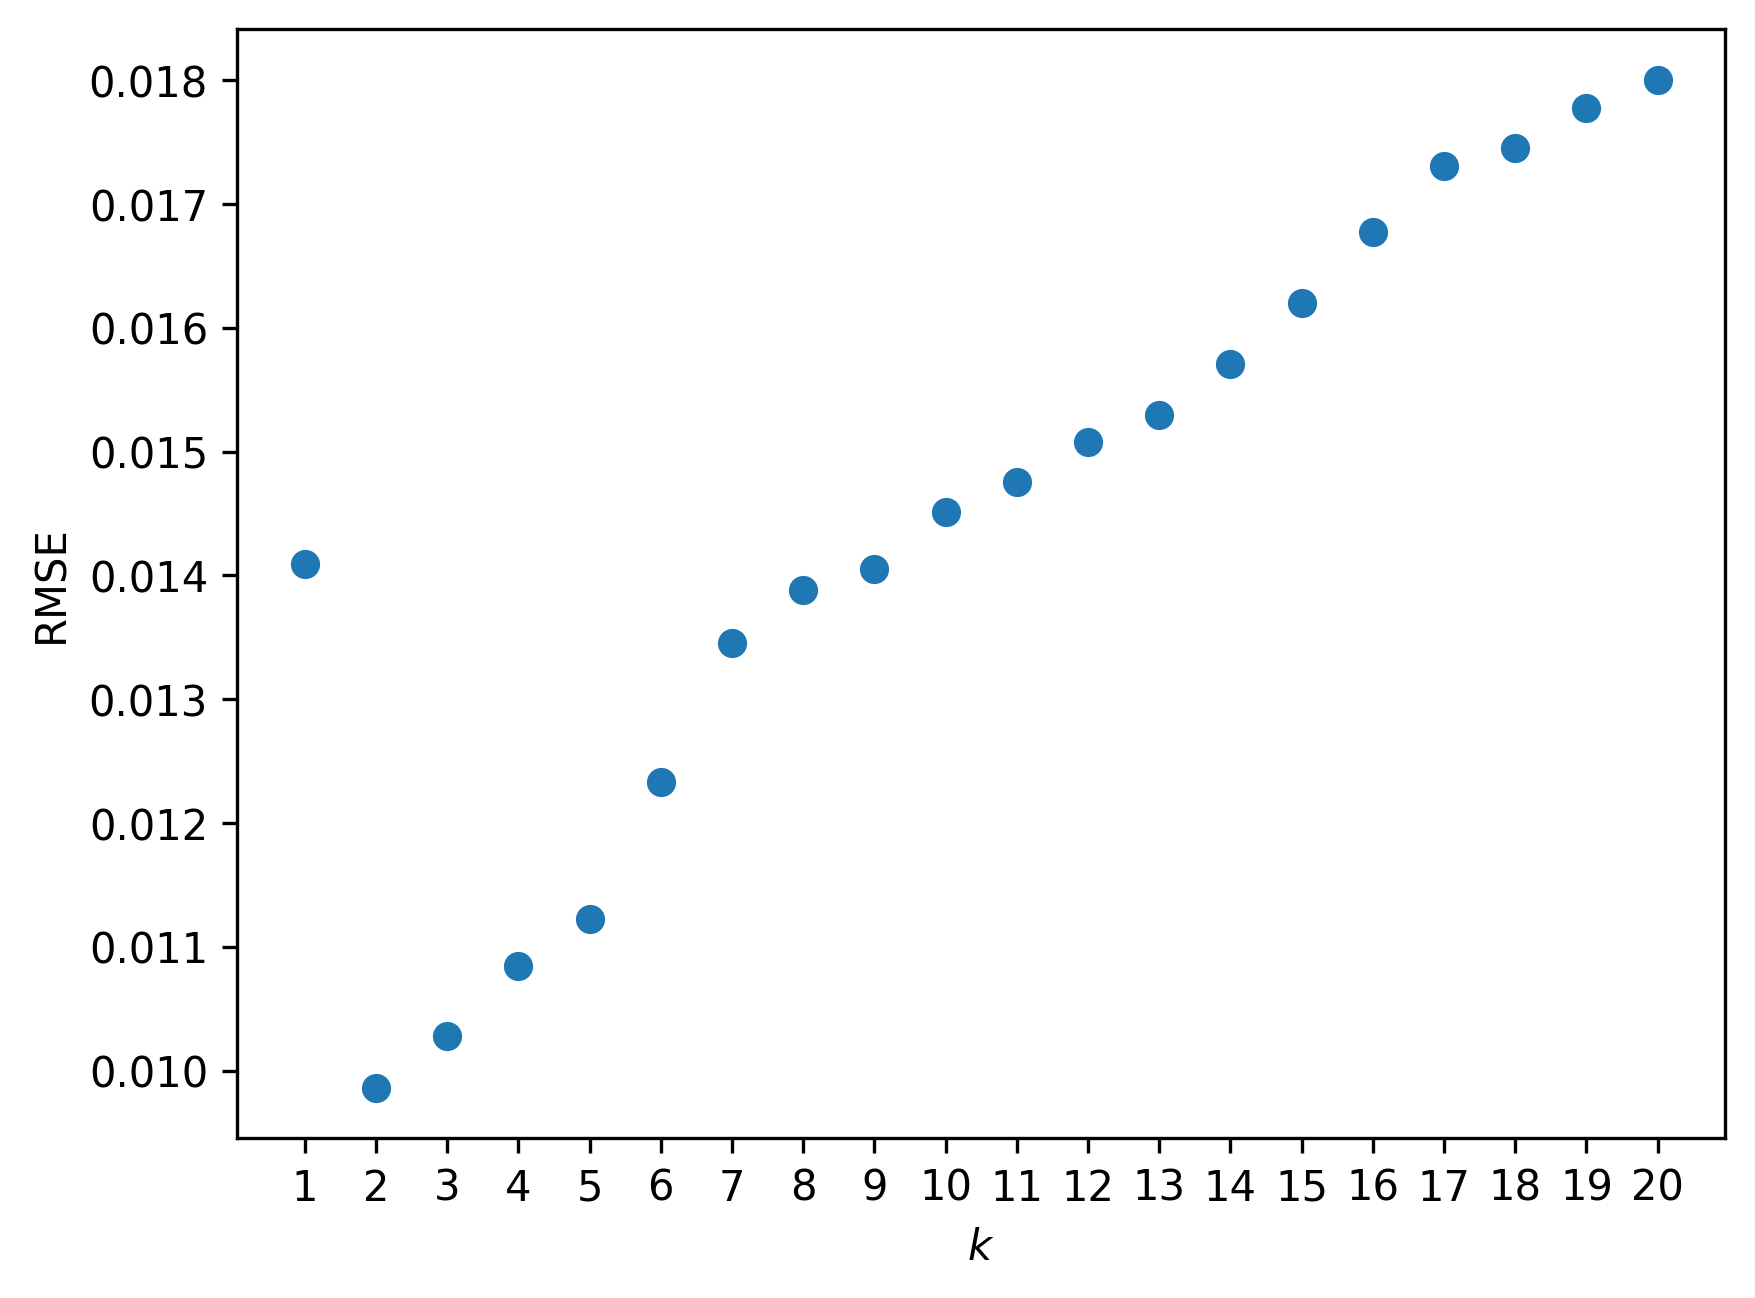
\includegraphics[width=0.5\textwidth]{graph/case3_knnr_rmse.png}
    \caption{$k$ hyperparameter-tuning of KNN regression model using RMSE in case 3}
    \label{fig:case3_knnr_rmse}
\end{figure}
We may plot the result of both linear regression and KNN regression in a form of surface over the range of the training data, which is shown in Figure \ref{fig:case3_lr_knnr_plane}. We can see that the linear regression model is not able to capture the non-linear relation between the inputs and the output.
\begin{figure}[H]
    \centering
    \begin{subfigure}{0.4\textwidth}
        \centering
        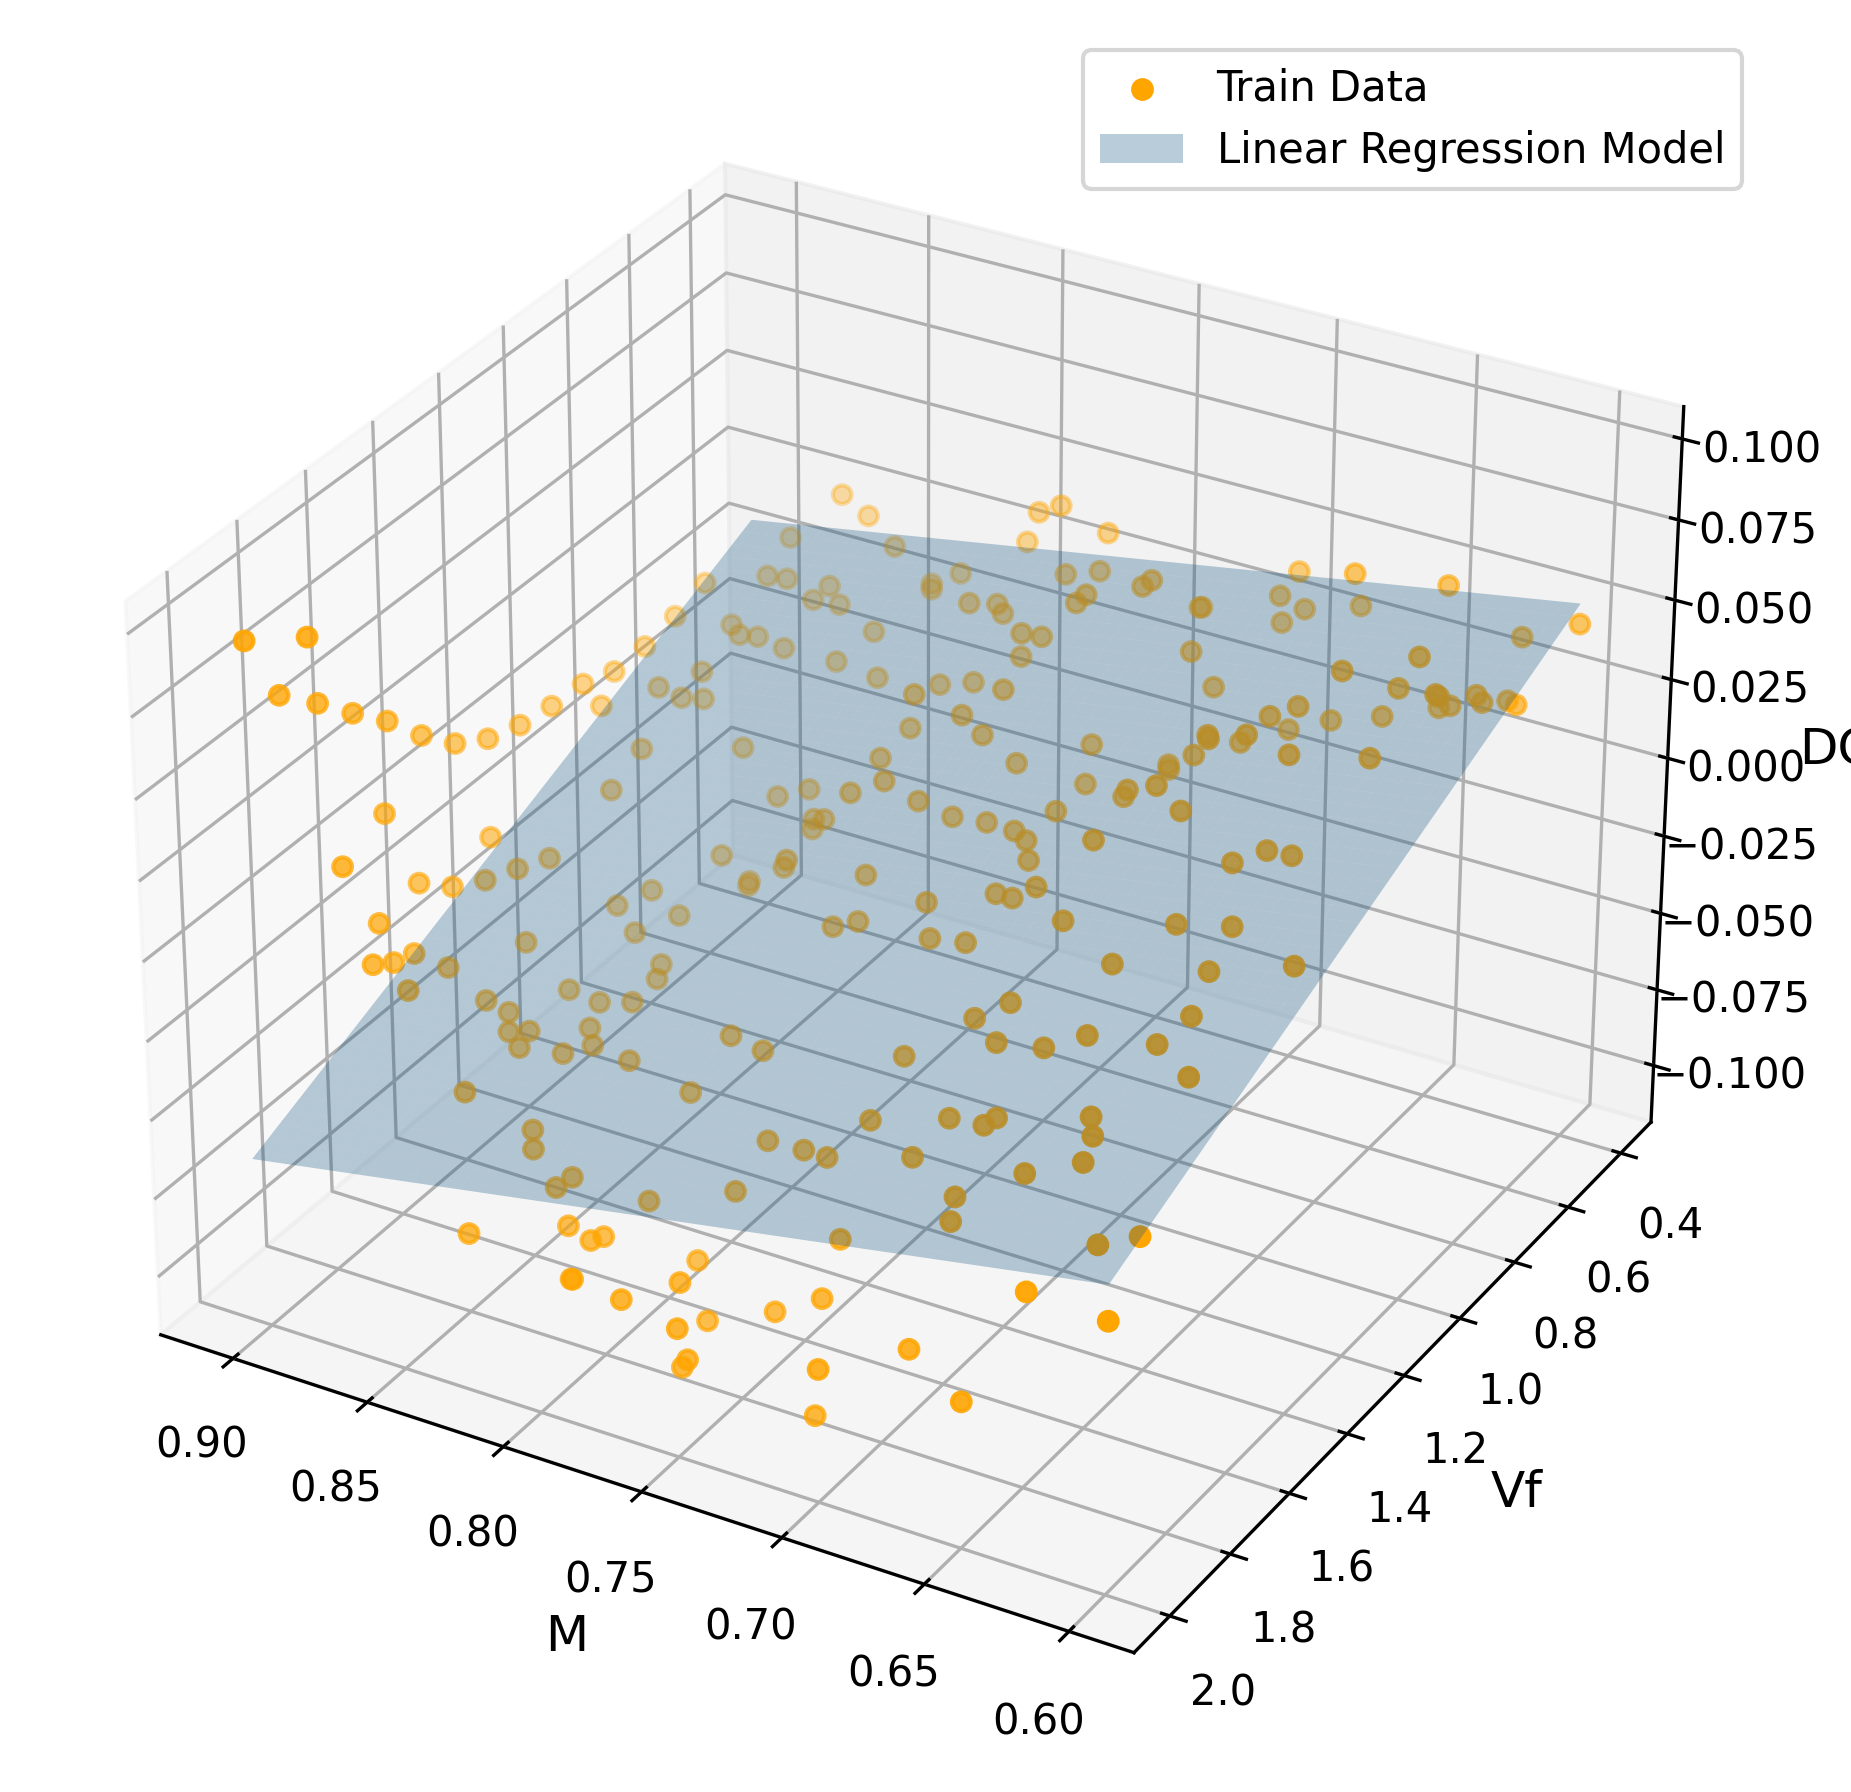
\includegraphics[width=1.0\textwidth]{graph/case3_lr_plane.png}
        \caption{Linear Regression}
    \end{subfigure}
    \hfill
    \begin{subfigure}{0.4\textwidth}
        \centering
        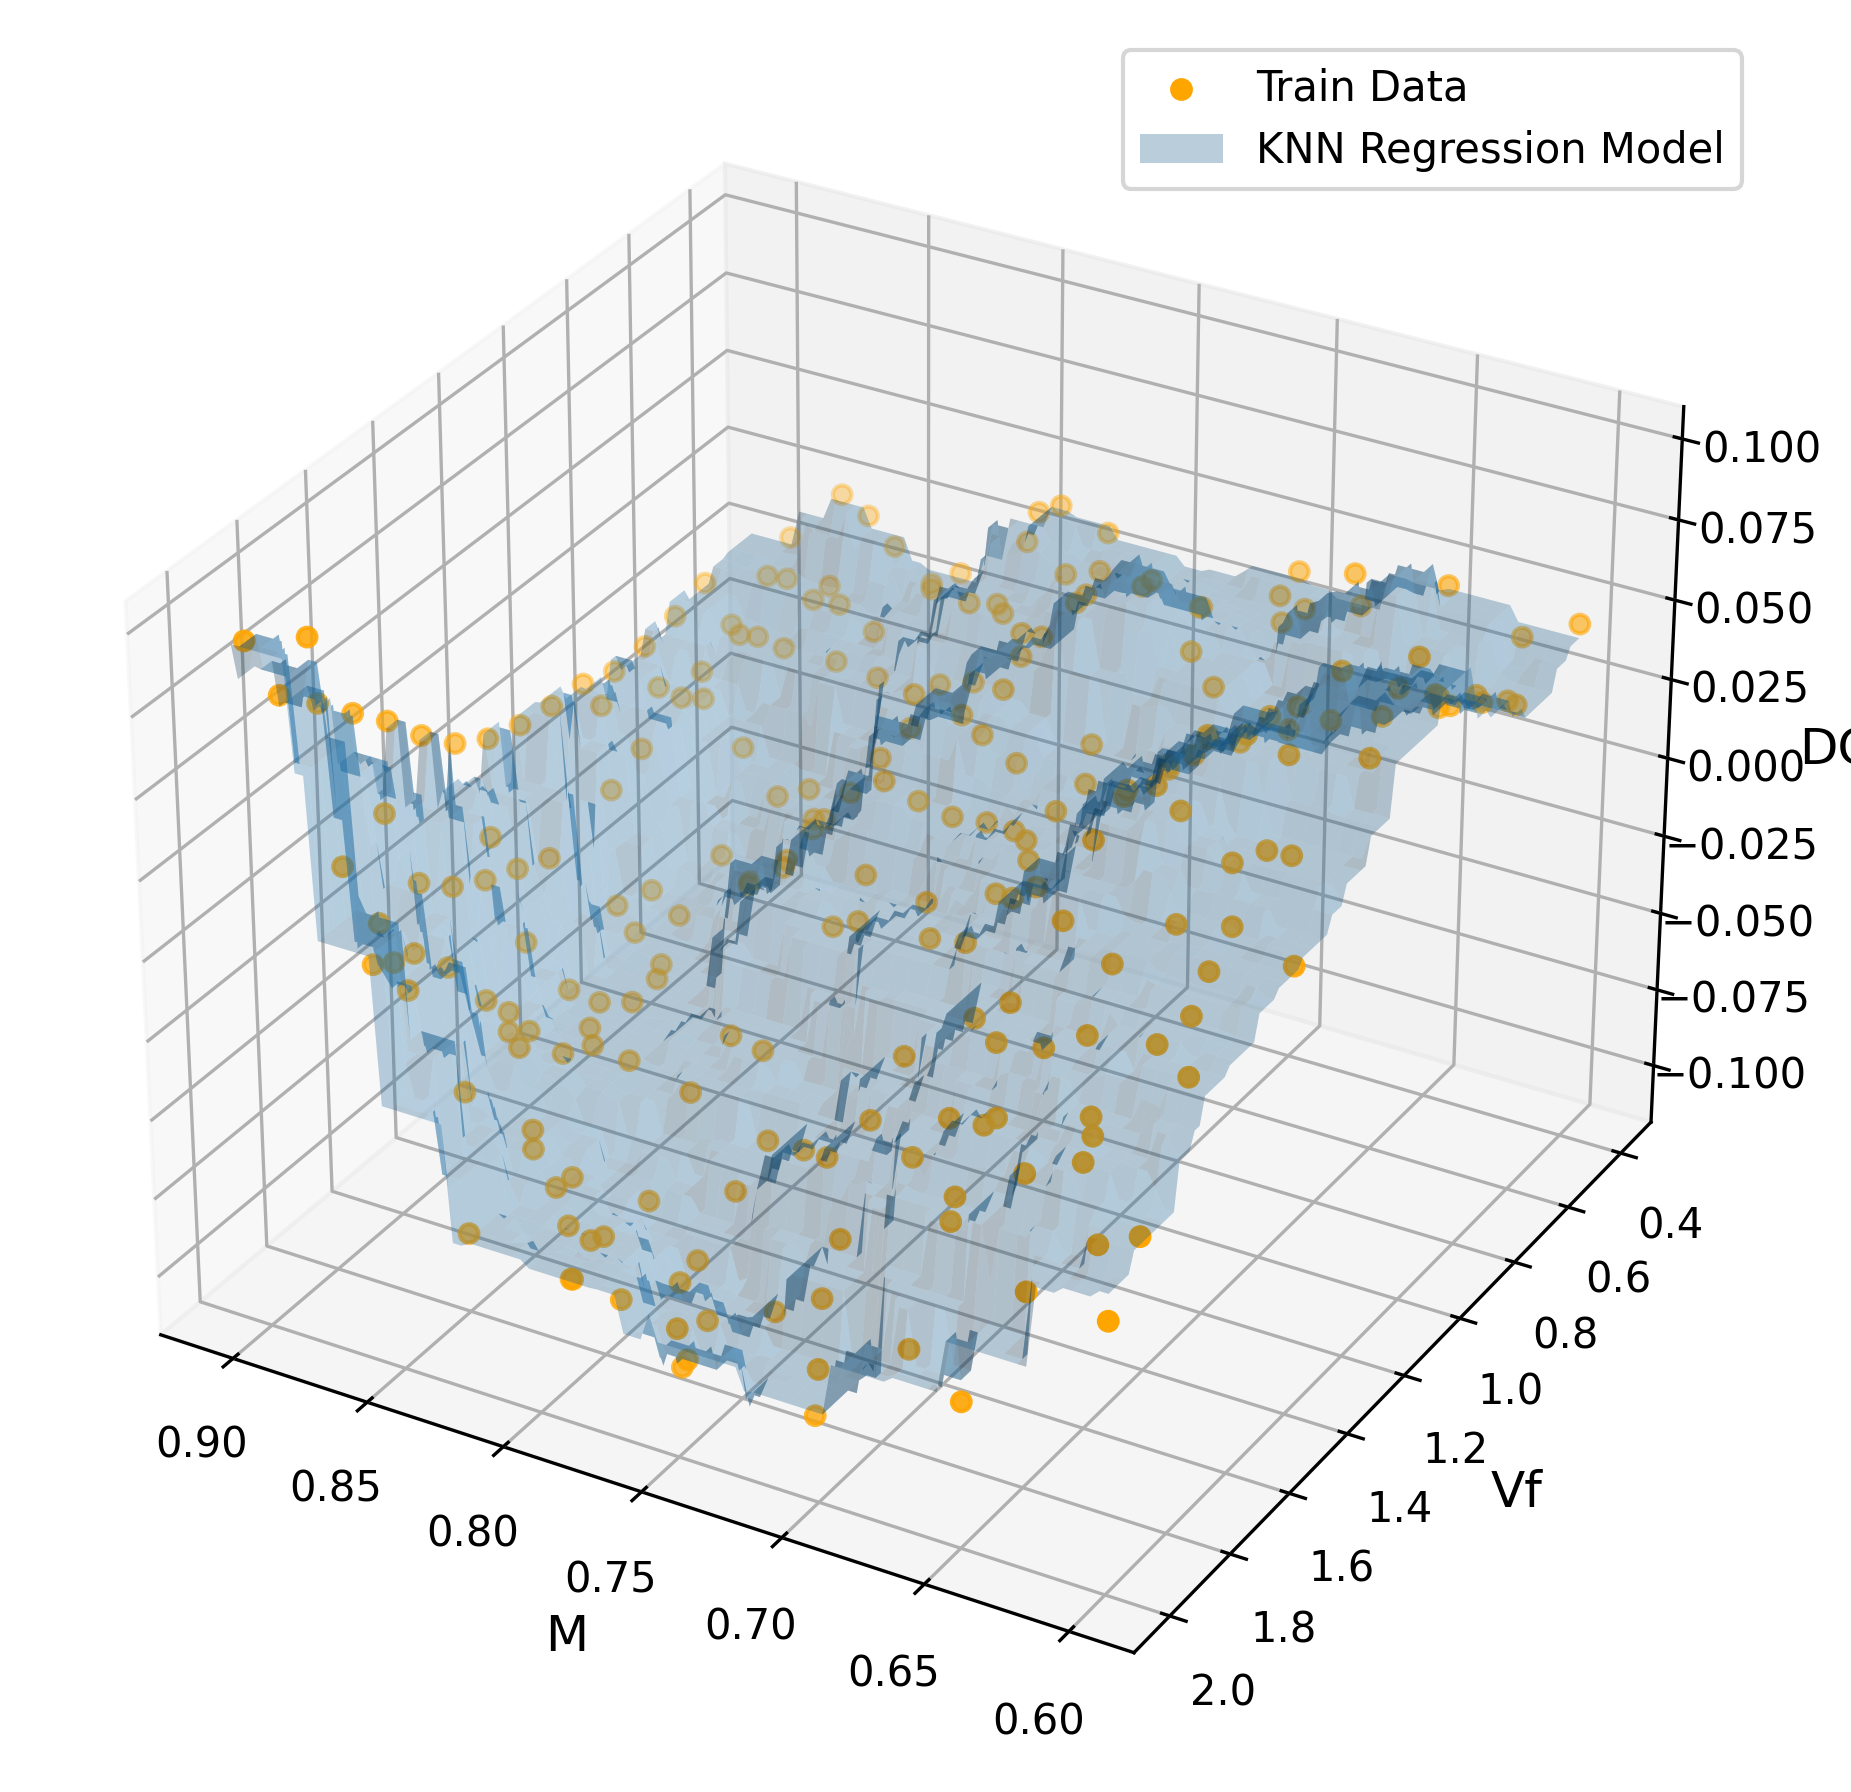
\includegraphics[width=1.0\textwidth]{graph/case3_knnr_plane.png}
        \caption{KNN Regression}
    \end{subfigure}

    \caption{Prediction surface of the regression model on training data in case 3 using (a) linear regression and (b) KNN regression}
    \label{fig:case3_lr_knnr_plane}
\end{figure}
After evaluating each model own parameters, we may now evaluate it with the testing data. The RMSE and MAE of the prediction is shown in Table \ref{tab:case3_lr_knnr_rmse_mae}, calculated using \texttt{mean\_squared\_error} and \texttt{mean\_absolute\_error} from \texttt{sklearn.metrics}. From there, we can see that the KNN regression model is able to predict the damping coefficient better than the linear regression model, as both the RMSE and MAE is lower than the linear regression model.
\begin{table}[H]
    \centering
    \caption{\label{tab:case3_lr_knnr_rmse_mae} RMSE and MAE of Linear Regression and KNN Regression in Case 3}
    \begin{tabular}{lrr}
        \toprule
        Model &      RMSE &       MAE \\
        \midrule
        Linear Regression &  0.029969 &  0.019001 \\
        KNN Regression    &  0.007907 &  0.005573 \\
        \bottomrule
    \end{tabular}
\end{table}

\subparagraph{Classification Model} We will use logistic regression and KNN classification to predict the flutter occurence. Using the algorithm of \eqref{eq:logregnewraph}, the resulting coefficient for the logistic regression model and the hypothesis testing is shown in Table \ref{tab:case3_logit_coef}. We can see that all $H_0$ is rejected and thus, all of the coefficients are significant. 
\begin{table}[H]
    \centering
    \caption{\label{tab:case3_logit_coef}Coefficient for Logistic Regression Model in Case 3}
    \begin{tabular}{lrrrrr}
        \toprule
        Beta &      Value &  Standard Error &  $t$-statistic &       $p$-value & Hypothesis Test Result \\
        \midrule
        0 &  0.158557 &        0.017985 &     8.816034 &  2.555677e-16 &              Reject $H_0$ \\
        1 & -0.145096 &        0.022156 &    -6.548710 &  3.543494e-10 &              Reject $H_0$ \\
        2 & -0.046859 &        0.004335 &   -10.808856 &  2.045755e-22 &              Reject $H_0$ \\
        \bottomrule
    \end{tabular}
\end{table}
Now, we may train our KNN classification model. Using 10-fold cross-validation, we obtained the best $k$ value of 3, taking F1-score as the scoring method. Figure \ref{fig:case3_knnc_f1} shows the result of the hyperparameter-tuning, and shows that the F1-score is the highest when $k=3$. 
\begin{figure}
    \centering
    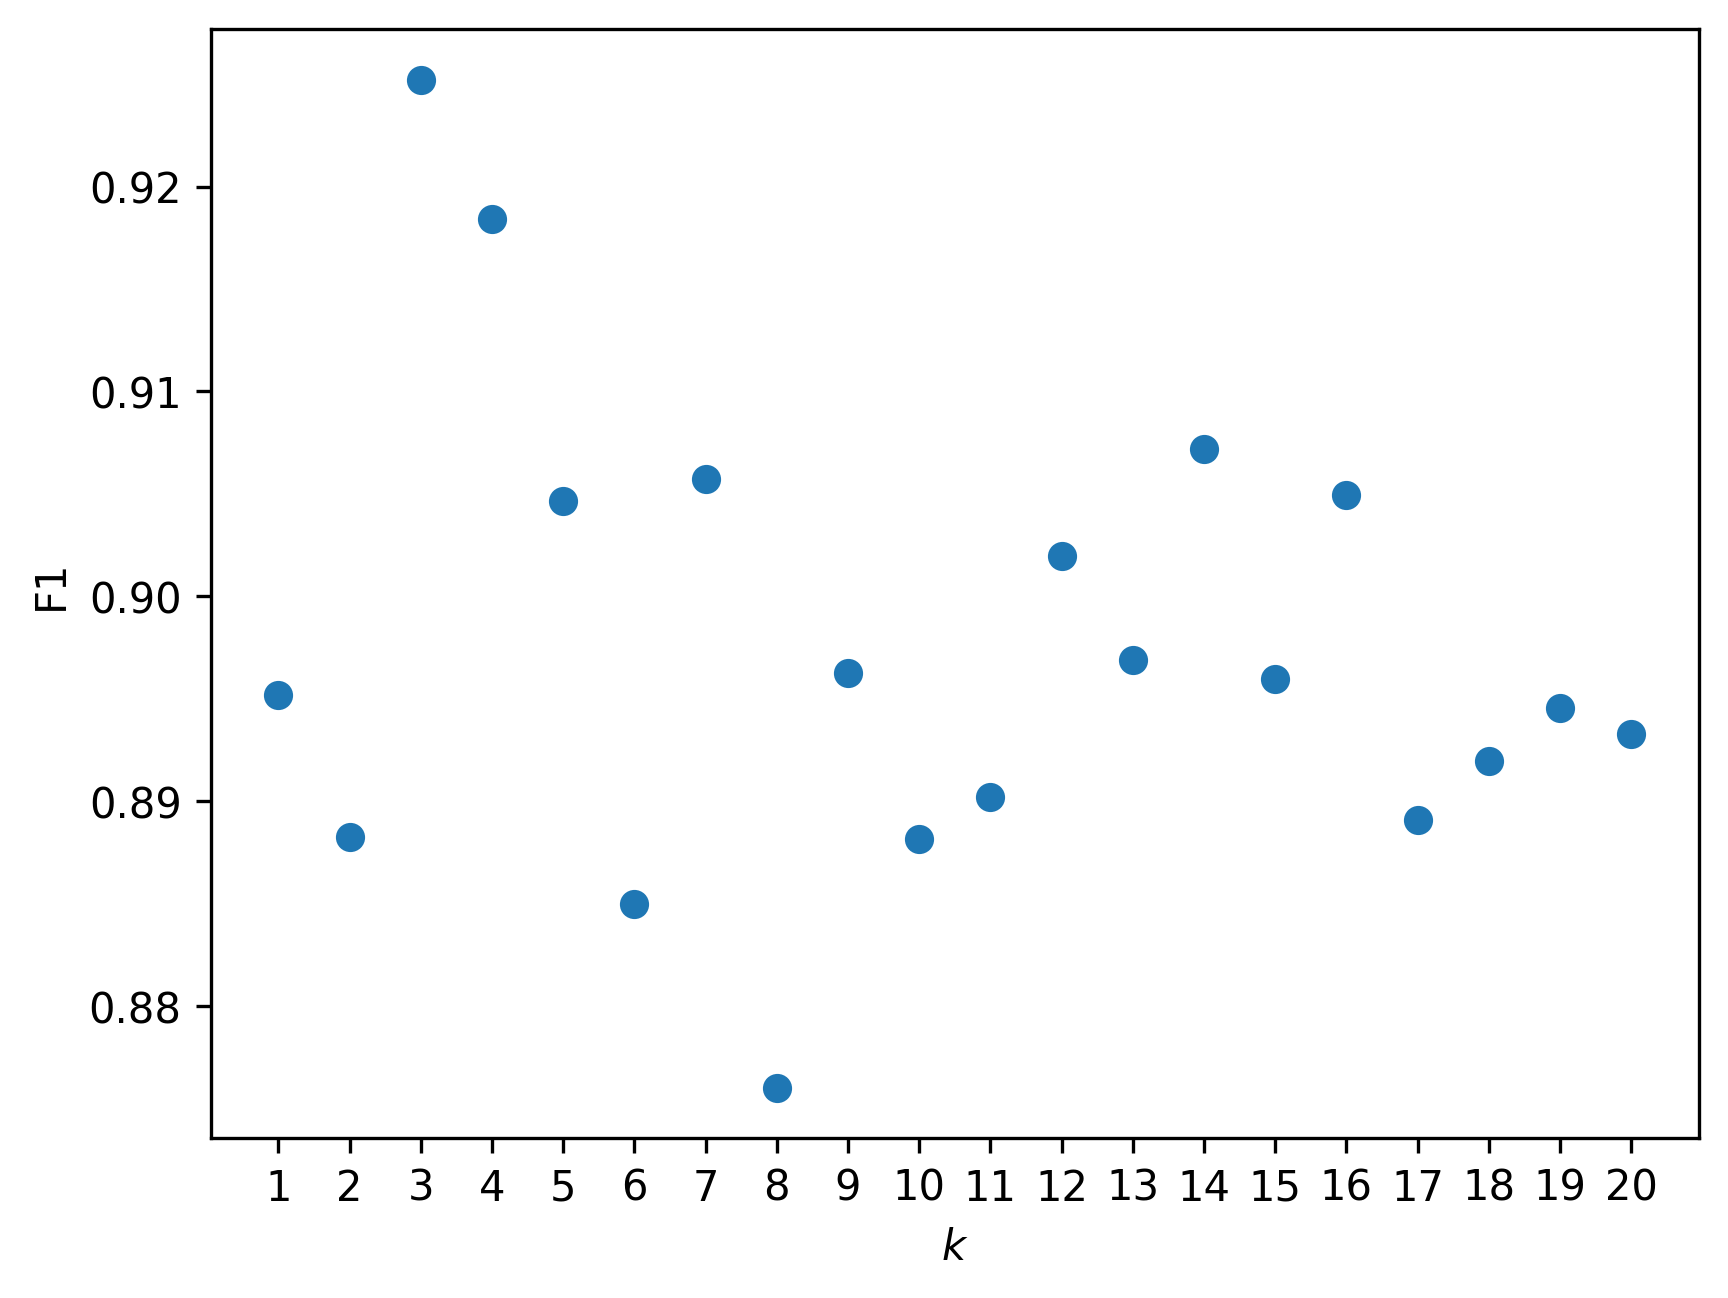
\includegraphics[width=0.5\textwidth]{graph/case3_knnc_f1.png}
    \caption{$k$ hyperparameter-tuning of KNN classification model using F1-score in case 3}
    \label{fig:case3_knnc_f1}
\end{figure}

\subparagraph{Model Evaluation} As we're dealing with a classification problem, we will use the scores of \eqref{eq:accuracy}, \eqref{eq:precision}, \eqref{eq:recall}, and \eqref{eq:f1score} to evaluate the model. The scores is calculated using \texttt{classification\_report} from \texttt{sklearn.metrics}. We will also provide the confusion matrix heatmap of the model to visualize more which how many data in each class is predicted right or wrong by the models. The result of the evaluation is shown in Table \ref{tab:case3_classification_report} and Figure \ref{fig:case3_confusion}.
\begin{figure}[H]
    \centering
    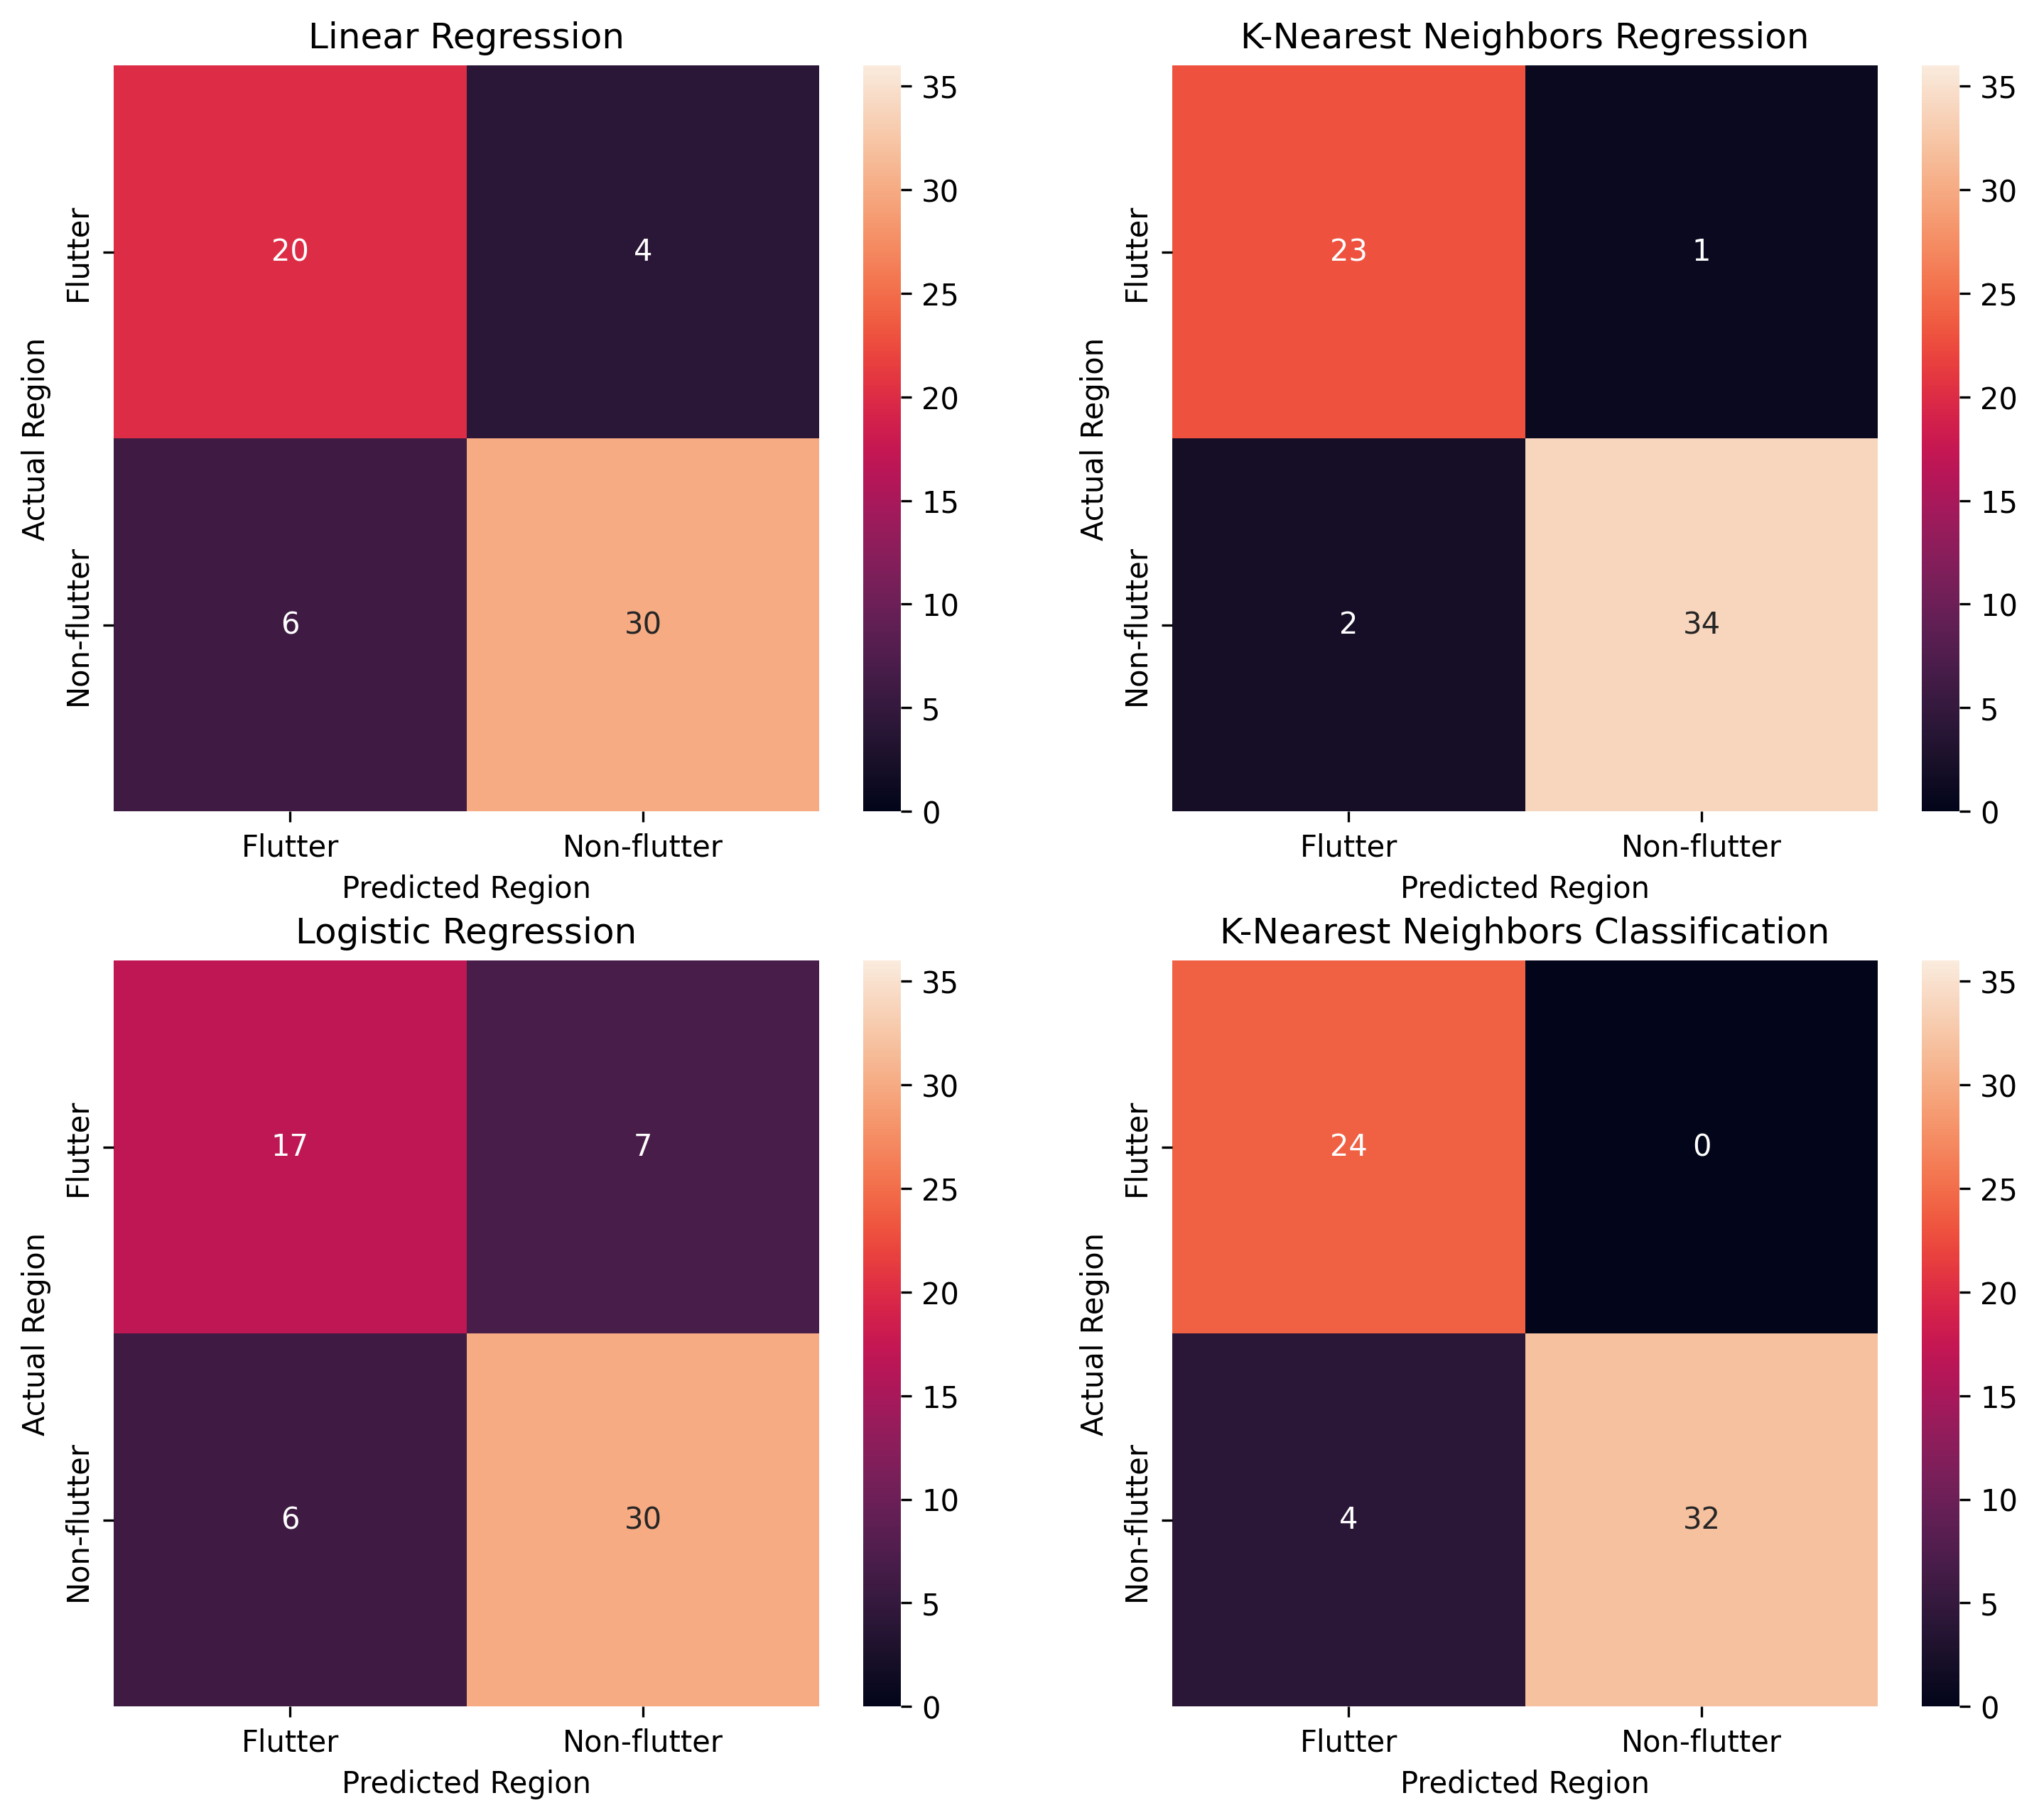
\includegraphics[width=1.0\textwidth]{graph/case3_confusion.png}
    \caption{Confusion matrix heatmap of the regression and classification model in case 3}
    \label{fig:case3_confusion}
\end{figure}

\begin{table}[H]
    \centering
    \caption{\label{tab:case3_classification_report}Classification report of the regression and classification model in case 3}
    \begin{tabular}{llrrrr}
        \toprule
        Model                               & Class         &  Precision    &  Recall       &  F1-score     & Accuracy \\
        \midrule
        \multirow{2}{*}{Linear Regression}  & Flutter       &  0.77         &  0.83         &  0.80         &  \multirow{2}{*}{0.83} \\
                                            & Non-flutter   &  0.88         &  0.83         &  0.86         &   \\
        \midrule
        \multirow{2}{*}{KNN Regression}     & Flutter       &  0.92         &  0.96         &  0.94         &  \multirow{2}{*}{0.95} \\
                                            & Non-flutter   &  0.97         &  0.94         &  0.96         &   \\
        \midrule
        \multirow{2}{*}{Logistic Regression} & Flutter       &  0.74         &  0.71         &  0.72         &  \multirow{2}{*}{0.78} \\
                                            & Non-flutter   &  0.81         &  0.83         &  0.82         &   \\
        \midrule
        \multirow{2}{*}{KNN Classification} & Flutter       &  0.86         &  1.00         &  0.92         &  \multirow{2}{*}{0.93} \\
                                            & Non-flutter   &  1.00         &  0.89         &  0.94         &   \\
        \bottomrule
    \end{tabular}
\end{table}
We can see that logistic regression model has the lowest accuracy, precision, recall, and F1-score. 

\paragraph{Conclusion} Our final result is the flutter boundary curve plotted in Figure \ref{fig:case3_boundary}. We can see that the linear regression and logistic regression model has a boundary in form of a line, while the KNN models have boundaries of a complex shape. This is as expected, as KNN is a non-parametric model, while linear regression and logistic regression are parametric models. For both KNN models, we can see that the region with large Mach is predicted poorly. This is due to the lack of data points provided by the dataset. To improve the result even more, we may find or add more data points to the dataset to increase its accuracy, tune the hyperparameter of KNN models, or even use more models, such as tree-based models and boosting algorithm models. 
\begin{figure}[H]
    \centering
    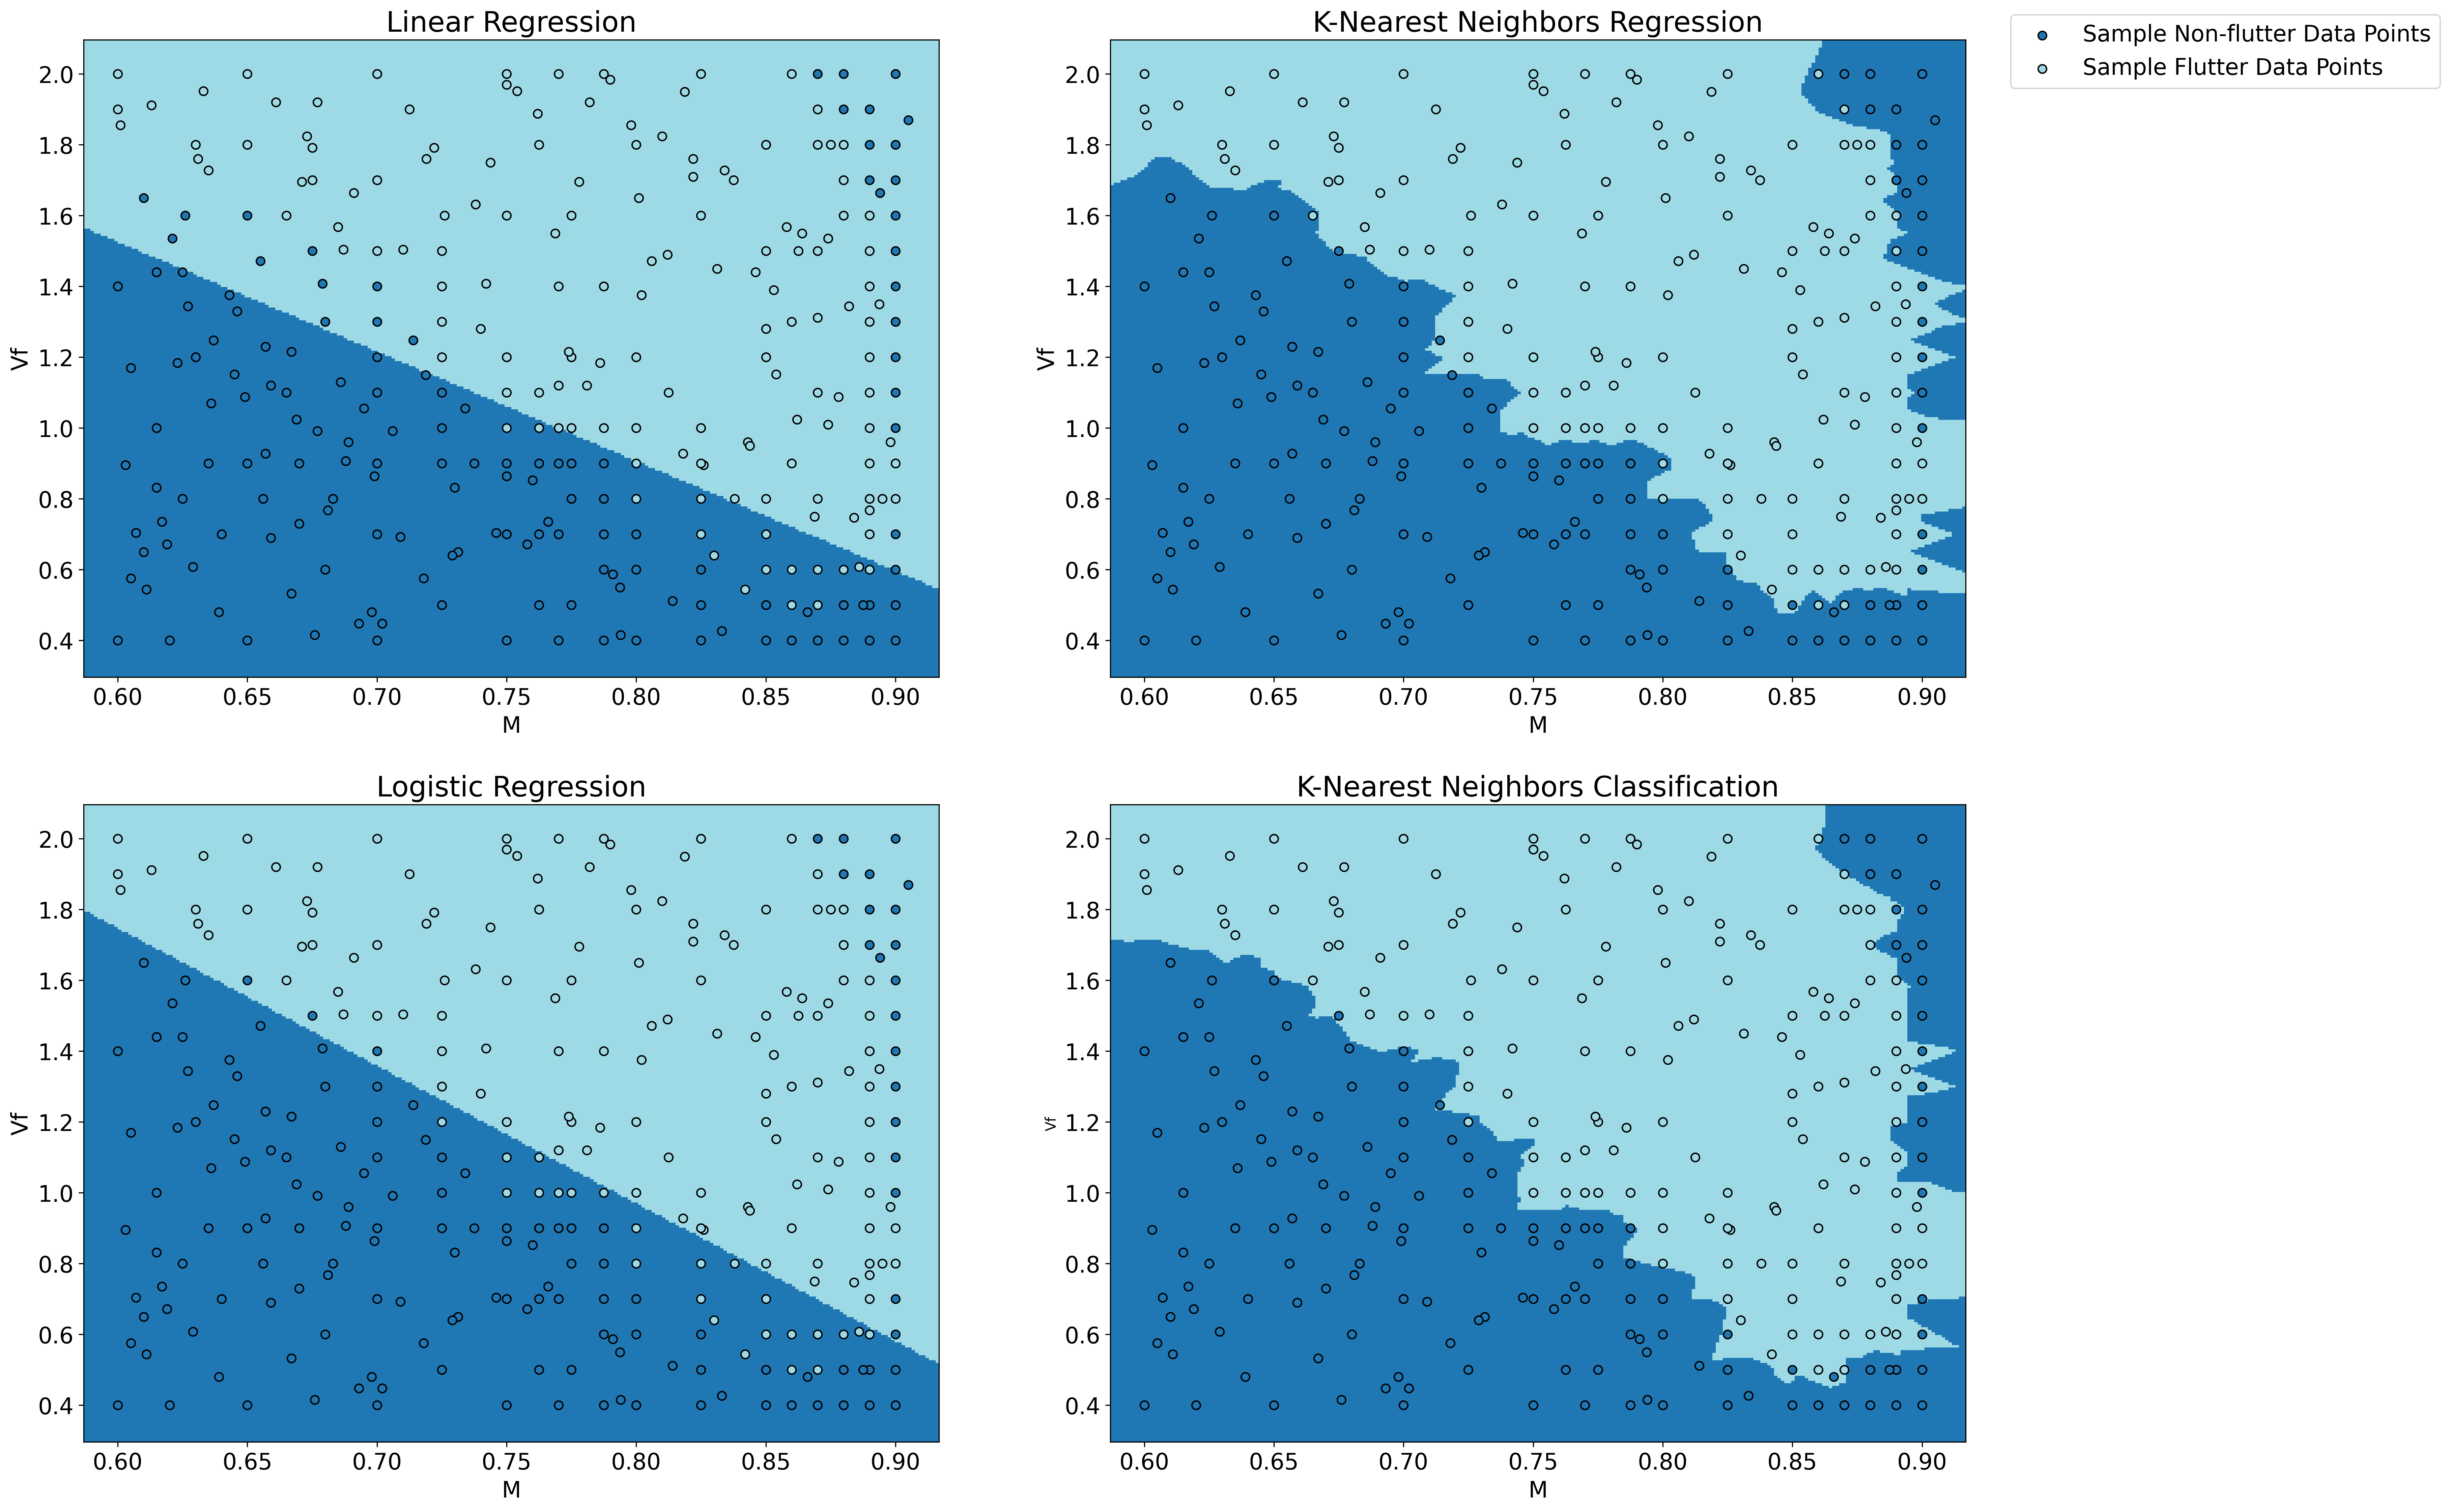
\includegraphics[width=1.0\textwidth]{graph/case3_boundary.png}
    \caption{Flutter boundary of the regression and classification model in case 3}
    \label{fig:case3_boundary}
\end{figure}

\section*{Appendix}

An Appendix, if needed, should appear before the acknowledgments.

\section*{Task Divisions}
\begin{table*}[H]
    \centering
    \caption{\label{tab:task_division}Task division of the project}
    \begin{tabular}{ll}
        \toprule
        Name & Task \\
        \midrule
        \multirow{2}{*}{Hafizh Renanto Akhmad} & Analysis of problem 3 \\
        & Put all answers together in the report \\
        \midrule
        \multirow{2}{*}{Isna Nur Firdausi} & Analysis of problem 1 \\
        & Model training and evaluation \\
        \midrule
        \multirow{2}{*}{Abisatya Hadyan Dhananjaya} & Analysis of problem 2, linear regression part \\
        & Model training and evaluation \\
        \midrule
        \multirow{2}{*}{Rizky Amalis Zhuraida} & Analysis of problem 2, KNN regression part \\
        & Model training and evaluation \\
        \bottomrule
    \end{tabular}
\end{table*}

\bibliographystyle{new-aiaa}
\bibliography{reference}

\end{document}
